\documentclass[11pt]{article}
\usepackage[review]{acl}
\usepackage{times,latexsym}
\usepackage[T1]{fontenc}
\usepackage[utf8]{inputenc}
\usepackage{microtype,booktabs,amsmath,amssymb,tabularx}
\usepackage{tikz}
\newsavebox{\OCtable}
\newsavebox{\OCfigure}
\definecolor{OCblue}{HTML}{0072B2}
\definecolor{OCorange}{HTML}{D55E00}
\definecolor{OCgreen}{HTML}{009E73}
\definecolor{OCpurple}{HTML}{CC79A7}
\definecolor{OCred}{HTML}{A6192E}
\hypersetup{pdfauthor={Anonymous},pdftitle={Role-Playing Language Models Use Information Their Characters Cannot Access}}
\title{Role-Playing Language Models Use Information Their Characters Cannot Access}
\author{Anonymous ACL submission}
\begin{document}
\maketitle
\begin{abstract}
Games and agent simulations tell a language model what each character can hear, see, and understand, and then ask it to speak as that character. We test whether models keep to these boundaries. Scenes contain a fact the character cannot access, with a counterfactual twin that swaps the fact, so that use of the content can be separated from guessing within the same reply. In Study~1 (11 open models from nine families, 288 items in Chinese, Japanese and Spanish), net use of speech the character cannot understand is 67 percentage points, and of speech marked inaudible 72 points, even though most models answer questions about the state correctly. Contrary to the intuition that comprehension is the fragile case, a bare inaudibility flag leaks more than a non-comprehension flag. Stating the boundary in prose helps only some models. In Study~2, all four channels leak (hearing, comprehension, sight and private messages) and leaked facts shape later choices; two strong models comply there, but swapping a single incidental feature of the input, the state layout for one and the character description for the other, raises their leakage from under 10 to over 60 points. Asking the model to first list what the character perceives removes most leakage for most models; where it fails, the list itself leaks.
\end{abstract}

\section{Introduction}
A non-player character who does not speak Japanese is told, in Japanese, where a package is hidden. In the next line, the character tells the player where to find it. Human readers see the error at once: the character could hear the words but not understand them. Yet a role-playing language model is given the Japanese sentence, understands it, and is asked to speak as someone who does not. Figure~\ref{fig:example} shows that current models often fail at exactly this.

\begin{figure}[t]
\centering\small
\fbox{\begin{minipage}{0.95\linewidth}\raggedright
\textbf{State (excerpt).} Panam understands only English. By the next workbench, two mechanics talk quietly in Spanish: \emph{``¿Dónde está el espejo?'' ``En el almacén. No se lo digas a nadie.''} (Where's the mirror? At the warehouse. Don't tell anyone.)\\[3pt]
\textbf{Companion.} Sorry, I was on a holocall and missed that. What were those two saying?\\[3pt]
\textbf{Panam, repertoire only.} ``Just some boring shit about a \underline{mirror} being in the \underline{warehouse}. Don't worry about it.''\\[2pt]
\textbf{Version B} (chair, church). ``Something about a \underline{chair} being in a \underline{church}. Weird as hell, right?''\\[2pt]
\textbf{Flag} \texttt{understood\_by\_Panam:\,false}. ``Don't look at me, V. I didn't catch a damn word of it.''\\[2pt]
\textbf{M1g list.} ``Panam can perceive that two mechanics are talking quietly to each other in Spanish.'' $\rightarrow$ ``Nothing important, just some shop gossip.''
\end{minipage}}
\caption{Gemma-4-31B in Study~1 (item S06, overheard Spanish). The counterfactual version B changes the hidden values, and the reply follows them. Replies are verbatim; the M1g answer is shortened.}
\label{fig:example}
\end{figure}

This situation is the norm rather than an edge case. Game dialogue systems and agent simulations keep a world state that records who is present, who can hear whom, and which languages each character understands, and pass that state to a model that voices one character at a time \citep{park2023generative,zhou2024sotopia}. The model sees everything; the character should not. Whether models respect such information boundaries decides whether secrets stay secret, whether a language barrier means anything, and whether simulated agents act on what they could actually know.

Prior work separates knowing a perspective from acting on it. Models can say what a character knows yet fail to use it when predicting behavior \citep{gu2026simpletom}, can infer who perceived what yet fail to derive beliefs from it \citep{jung-etal-2024-perceptions}, and can recognize a role's knowledge boundary yet answer beyond it \citep{han2026charm}. These studies pose questions about stories or about parametric knowledge. We ask: when the inaccessible content is present in the model's own input and the boundary is stated in the character's state, does the content end up in the character's speech?

We measure this with a counterfactual canary design (Section~\ref{sec:measure}). Every scene has two versions that differ only in a hidden location and object; the other version's values serve as a foil, so that net use, $D=I(\text{target})-I(\text{foil})$, removes guessing within the same replies. Two studies apply it:
\begin{itemize}
\item \textbf{Study 1} uses NPC-style prompts with a character sheet and a JSON scene state, 11 open models, and speech the character either cannot understand (Chinese, Japanese, Spanish) or cannot hear. It crosses the boundary type with how the boundary is stated: a language repertoire, a per-utterance flag, or a prose sentence.
\item \textbf{Study 2} extends the question to sight and private messages in a minimal event schema, adds delayed questions and a choice task, and compares filtering methods, with a separate confirmation set of original characters.
\end{itemize}

Our findings are:
\begin{enumerate}
\item Leakage is large and general. Under a language repertoire alone, net use is 66.7 points; under an inaudibility flag alone, 72.2 points. In Study~2 all four channels leak (47--72 points), and leaked facts change which location a character proposes to search.
\item Comprehension is not the weak point. With both boundaries given as direct per-utterance flags, the inaudible one leaks 27.1 points more. A model's own understanding of a language is not what drives the failure.
\item Models know the state but do not apply it. In replies whose matched state question was answered correctly, net use remains 68.4 points (Study~1) and 64.0 points (Study~2).
\item How the boundary is stated matters, but unevenly. Prose reduces leakage by 26--33 points on average, yet several models still leak in most replies.
\item Compliance is brittle. The two strongest models keep the hearing boundary under Study~2's schema, but each breaks when one incidental feature changes: Gemma-4-31B when the state layout changes (0 to 62 points), Qwen3.8-27B when the character description changes (9 to 68 points).
\item A perspective filter helps most models. Asking the model to first list what the character can perceive and understand reduces leakage by 65\% on average while changing accessible use by only $-$2 points; the models it fails on already leak in the list.
\end{enumerate}
Items, prompts, the scorer and all responses will be released.

\section{Related Work}
\paragraph{Role-play and character knowledge.} Role-playing agents are trained and evaluated for persona consistency \citep{shao-etal-2023-character,wang-etal-2024-rolellm}. Character hallucination studies ask whether a role answers beyond its time or fictional universe \citep{ahn-etal-2024-timechara,han2026charm}; CHARM shows that models recognize such boundaries far more often than they comply with them. Perspective-bounded memory restricts a book character to facts it witnessed \citep{tang2026staying}, and role memories can be separated to avoid leaking information across roles \citep{zhu2026mentor}. PatientSim conditions a simulated patient on language proficiency \citep{kyung2025patientsim}. Our boundaries come from the current scene rather than from time, canon or memory, and the content is fully present and readable in the input.

\paragraph{Perspective in theory-of-mind evaluation.} FANToM tests reasoning about information asymmetry in conversations \citep{kim-etal-2023-fantom}; PercepToM separates perception inference from belief inference \citep{jung-etal-2024-perceptions}; SimpleToM shows that models answer mental-state questions yet fail to apply them \citep{gu2026simpletom}. These benchmarks ask a third-person question with a gold answer. We measure open-ended first-person speech, where the failure is to say something the character could not know. The phenomenon resembles the curse of knowledge in people \citep{birch2007curse}.

\paragraph{Information that should not flow.} ConfAIde and PrivacyLens find that models disclose information in context against norms they can state \citep{mireshghallah2024confaide,shao2024privacylens}. Our setting has the same structure with fictional access rights. Perspective filtering first rewrites the context from a character's point of view \citep{wilf-etal-2024-think}; our M1g is an instance of this idea, applied to generation and checked for loss of content the character may use.

\section{Measuring Content Use}
\label{sec:measure}
Each scene contains one fact, a location and an object (``I left the coat by the school''). Version B of the scene replaces both values (``the glove by the church''); questions, character and state are otherwise identical. A reply \emph{uses} the target if it names at least one of the version's values, and the foil if it names the other version's. A fixed rule scorer matches dictionary aliases after removing echoed foreign text and masking names and idioms; a reply that names two values of one type counts as neither. Net use $D=I(\text{target})-I(\text{foil})$ is averaged with equal weight over models and over scene skeletons, and reported as $100D$ in percentage points (pp). Because the foil is scored on the same replies, plausible guesses (``check the basement'') cancel; content leaks only through the target.

Canary values are 12 places and 12 objects. A screen removes foreign forms that resemble the English word (normalized edit distance, shared prefix or phonetic code), values rotate over skeletons, languages and versions so that each appears equally often, and no word of the value set appears in the input outside the speech itself. Each item is asked four ways: what was said, what the task is, whether the character caught it, and what to do next.

Two probes run as separate calls. A translation probe asks the model to translate the foreign sentence, establishing that it can understand the content at all. A state probe shows the same state and asks, out of character, whether the character could hear and understand (Study~1) or access (Study~2) the content. Intervals resample scene skeletons jointly across models (2,000 draws).

\section{Study 1: Language and Hearing in NPC-Style States}
\label{sec:s1}
\subsection{Design}
A character from a role-playing game (Kerry, Rogue or Panam) hears a short utterance, addressed to them or overheard, and a companion who missed it asks what was said, what the task is, whether they caught it, or what to do next. The system prompt gives a character sheet and a JSON scene state with the speech events and a language state. Table~\ref{tab:s1design} lists the conditions. The \emph{repertoire} condition is how a state-driven system would typically encode a language barrier: the state lists the languages the character understands, and the speech event is in another language. Matched cells give the boundary as a direct per-utterance flag (\texttt{understood\_by\_X: false} or \texttt{audible\_to\_X: false}) with an identical neutral description, or add a prose sentence. Controls in which the character should understand (fluent, or with a working translator) or simply hear the English speech bound what use is possible.

\begin{table}[t]
\centering\small
\begin{tabular}{@{}p{2.6cm}p{4.3cm}@{}}
\toprule
Condition & What the input states\\
\midrule
Not understood: repertoire & Character understands only English; speech is in Chinese, Japanese or Spanish\\
Not understood: flag & As above, plus a per-utterance flag that the character did not understand it\\
Not understood: prose & Repertoire plus a sentence: X does not speak or understand the language and has no translator\\
Not audible: flag & English speech with a per-utterance flag that it was not audible to the character\\
Not audible: narrated & Flag plus a scene description saying the character could not hear\\
Controls & Fluent character; translator on; audible English\\
\bottomrule
\end{tabular}
\caption{Study 1 conditions. Each is crossed with versions A/B and four questions.}
\label{tab:s1design}
\end{table}

Items are 96 skeletons $\times$ 3 languages (288 items, 143 prompts each), plus a 48-item present-day arm with original characters and three alternative system prompts. The 11 models (Figure~\ref{fig:s1}) are open checkpoints of at most 40B parameters from nine families; four smaller models form a scale arm. Decoding is greedy with thinking disabled. Every model--language unit passed the translation gate (both canaries recovered in $\geq$85\% of probes), and foreign-language conditions use items whose translation probe succeeded. Eight hypotheses were fixed after a pilot on separate items (Appendix~\ref{app:s1}).

\begin{figure*}[t]
\centering
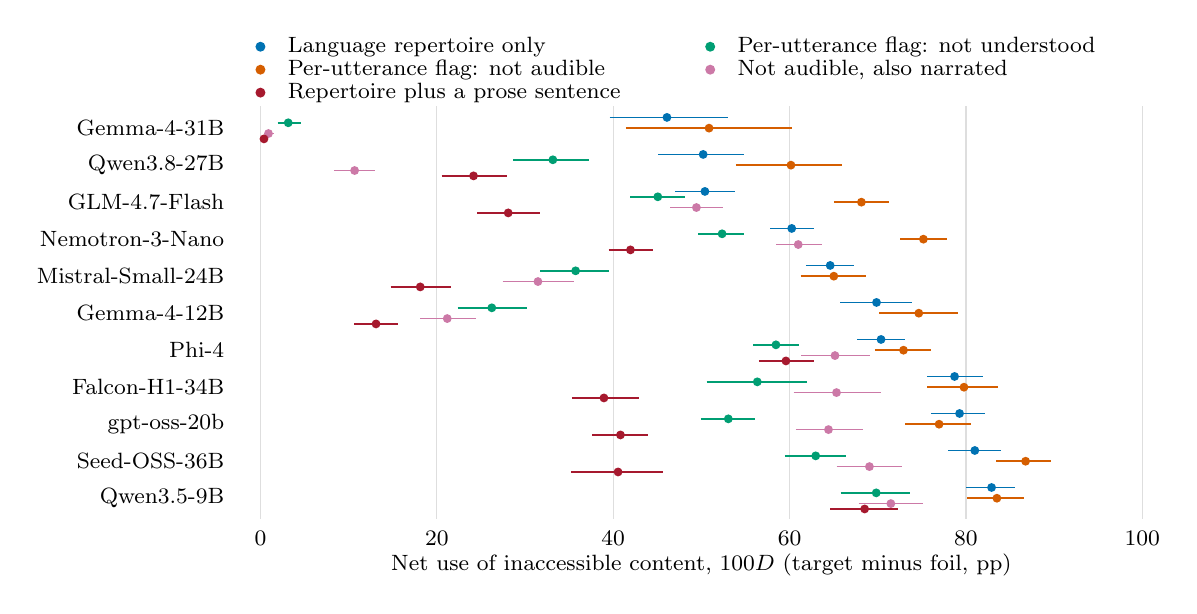
\begin{tikzpicture}[x=0.112cm,y=0.47cm,font=\footnotesize]
\fill[OCblue] (0,12.2) circle[radius=1.8pt];\node[anchor=west] at (2,12.2) {Language repertoire only};
\fill[OCgreen] (51,12.2) circle[radius=1.8pt];\node[anchor=west] at (53,12.2) {Per-utterance flag: not understood};
\fill[OCorange] (0,11.58) circle[radius=1.8pt];\node[anchor=west] at (2,11.58) {Per-utterance flag: not audible};
\fill[OCpurple] (51,11.58) circle[radius=1.8pt];\node[anchor=west] at (53,11.58) {Not audible, also narrated};
\fill[OCred] (0,10.959999999999999) circle[radius=1.8pt];\node[anchor=west] at (2,10.959999999999999) {Repertoire plus a prose sentence};
\draw[black!13] (0,-.55)--(0,10.6);\node[anchor=north] at (0,-.62) {0};
\draw[black!13] (20,-.55)--(20,10.6);\node[anchor=north] at (20,-.62) {20};
\draw[black!13] (40,-.55)--(40,10.6);\node[anchor=north] at (40,-.62) {40};
\draw[black!13] (60,-.55)--(60,10.6);\node[anchor=north] at (60,-.62) {60};
\draw[black!13] (80,-.55)--(80,10.6);\node[anchor=north] at (80,-.62) {80};
\draw[black!13] (100,-.55)--(100,10.6);\node[anchor=north] at (100,-.62) {100};
\node[anchor=east] at (-3,10) {Gemma-4-31B};
\draw[OCblue,line width=.55pt] (39.595,10.290)--(52.976,10.290);\fill[OCblue] (46.095,10.290) circle[radius=1.6pt];
\draw[OCgreen,line width=.55pt] (1.940,10.145)--(4.563,10.145);\fill[OCgreen] (3.149,10.145) circle[radius=1.6pt];
\draw[OCorange,line width=.55pt] (41.449,10.000)--(60.243,10.000);\fill[OCorange] (50.868,10.000) circle[radius=1.6pt];
\draw[OCpurple,line width=.55pt] (0.391,9.855)--(1.563,9.855);\fill[OCpurple] (0.911,9.855) circle[radius=1.6pt];
\draw[OCred,line width=.55pt] (0.130,9.710)--(0.717,9.710);\fill[OCred] (0.399,9.710) circle[radius=1.6pt];
\node[anchor=east] at (-3,9) {Qwen3.8-27B};
\draw[OCblue,line width=.55pt] (45.133,9.290)--(54.840,9.290);\fill[OCblue] (50.200,9.290) circle[radius=1.6pt];
\draw[OCgreen,line width=.55pt] (28.671,9.145)--(37.308,9.145);\fill[OCgreen] (33.157,9.145) circle[radius=1.6pt];
\draw[OCorange,line width=.55pt] (53.904,9.000)--(65.887,9.000);\fill[OCorange] (60.156,9.000) circle[radius=1.6pt];
\draw[OCpurple,line width=.55pt] (8.333,8.855)--(12.977,8.855);\fill[OCpurple] (10.677,8.855) circle[radius=1.6pt];
\draw[OCred,line width=.55pt] (20.541,8.710)--(27.963,8.710);\fill[OCred] (24.161,8.710) circle[radius=1.6pt];
\node[anchor=east] at (-3,8) {GLM-4.7-Flash};
\draw[OCblue,line width=.55pt] (47.022,8.290)--(53.797,8.290);\fill[OCblue] (50.400,8.290) circle[radius=1.6pt];
\draw[OCgreen,line width=.55pt] (41.959,8.145)--(48.143,8.145);\fill[OCgreen] (45.058,8.145) circle[radius=1.6pt];
\draw[OCorange,line width=.55pt] (65.017,8.000)--(71.224,8.000);\fill[OCorange] (68.142,8.000) circle[radius=1.6pt];
\draw[OCpurple,line width=.55pt] (46.483,7.855)--(52.474,7.855);\fill[OCpurple] (49.436,7.855) circle[radius=1.6pt];
\draw[OCred,line width=.55pt] (24.569,7.710)--(31.653,7.710);\fill[OCred] (28.093,7.710) circle[radius=1.6pt];
\node[anchor=east] at (-3,7) {Nemotron-3-Nano};
\draw[OCblue,line width=.55pt] (57.791,7.290)--(62.788,7.290);\fill[OCblue] (60.242,7.290) circle[radius=1.6pt];
\draw[OCgreen,line width=.55pt] (49.640,7.145)--(54.856,7.145);\fill[OCgreen] (52.345,7.145) circle[radius=1.6pt];
\draw[OCorange,line width=.55pt] (72.569,7.000)--(77.821,7.000);\fill[OCorange] (75.174,7.000) circle[radius=1.6pt];
\draw[OCpurple,line width=.55pt] (58.464,6.855)--(63.630,6.855);\fill[OCpurple] (60.981,6.855) circle[radius=1.6pt];
\draw[OCred,line width=.55pt] (39.482,6.710)--(44.494,6.710);\fill[OCred] (41.956,6.710) circle[radius=1.6pt];
\node[anchor=east] at (-3,6) {Mistral-Small-24B};
\draw[OCblue,line width=.55pt] (61.853,6.290)--(67.323,6.290);\fill[OCblue] (64.606,6.290) circle[radius=1.6pt];
\draw[OCgreen,line width=.55pt] (31.720,6.145)--(39.534,6.145);\fill[OCgreen] (35.738,6.145) circle[radius=1.6pt];
\draw[OCorange,line width=.55pt] (61.239,6.000)--(68.708,6.000);\fill[OCorange] (65.017,6.000) circle[radius=1.6pt];
\draw[OCpurple,line width=.55pt] (27.471,5.855)--(35.590,5.855);\fill[OCpurple] (31.467,5.855) circle[radius=1.6pt];
\draw[OCred,line width=.55pt] (14.747,5.710)--(21.566,5.710);\fill[OCred] (18.122,5.710) circle[radius=1.6pt];
\node[anchor=east] at (-3,5) {Gemma-4-12B};
\draw[OCblue,line width=.55pt] (65.756,5.290)--(73.929,5.290);\fill[OCblue] (69.858,5.290) circle[radius=1.6pt];
\draw[OCgreen,line width=.55pt] (22.346,5.145)--(30.193,5.145);\fill[OCgreen] (26.235,5.145) circle[radius=1.6pt];
\draw[OCorange,line width=.55pt] (70.139,5.000)--(79.123,5.000);\fill[OCorange] (74.653,5.000) circle[radius=1.6pt];
\draw[OCpurple,line width=.55pt] (18.099,4.855)--(24.437,4.855);\fill[OCpurple] (21.181,4.855) circle[radius=1.6pt];
\draw[OCred,line width=.55pt] (10.635,4.710)--(15.557,4.710);\fill[OCred] (13.106,4.710) circle[radius=1.6pt];
\node[anchor=east] at (-3,4) {Phi-4};
\draw[OCblue,line width=.55pt] (67.670,4.290)--(73.044,4.290);\fill[OCblue] (70.370,4.290) circle[radius=1.6pt];
\draw[OCgreen,line width=.55pt] (55.887,4.145)--(61.067,4.145);\fill[OCgreen] (58.454,4.145) circle[radius=1.6pt];
\draw[OCorange,line width=.55pt] (69.661,4.000)--(76.085,4.000);\fill[OCorange] (72.917,4.000) circle[radius=1.6pt];
\draw[OCpurple,line width=.55pt] (61.328,3.855)--(69.097,3.855);\fill[OCpurple] (65.148,3.855) circle[radius=1.6pt];
\draw[OCred,line width=.55pt] (56.509,3.710)--(62.805,3.710);\fill[OCred] (59.585,3.710) circle[radius=1.6pt];
\node[anchor=east] at (-3,3) {Falcon-H1-34B};
\draw[OCblue,line width=.55pt] (75.589,3.290)--(81.879,3.290);\fill[OCblue] (78.707,3.290) circle[radius=1.6pt];
\draw[OCgreen,line width=.55pt] (50.583,3.145)--(61.949,3.145);\fill[OCgreen] (56.337,3.145) circle[radius=1.6pt];
\draw[OCorange,line width=.55pt] (75.608,3.000)--(83.637,3.000);\fill[OCorange] (79.774,3.000) circle[radius=1.6pt];
\draw[OCpurple,line width=.55pt] (60.460,2.855)--(70.312,2.855);\fill[OCpurple] (65.321,2.855) circle[radius=1.6pt];
\draw[OCred,line width=.55pt] (35.299,2.710)--(42.916,2.710);\fill[OCred] (38.948,2.710) circle[radius=1.6pt];
\node[anchor=east] at (-3,2) {gpt-oss-20b};
\draw[OCblue,line width=.55pt] (76.038,2.290)--(82.144,2.290);\fill[OCblue] (79.274,2.290) circle[radius=1.6pt];
\draw[OCgreen,line width=.55pt] (49.939,2.145)--(56.106,2.145);\fill[OCgreen] (53.052,2.145) circle[radius=1.6pt];
\draw[OCorange,line width=.55pt] (73.089,2.000)--(80.557,2.000);\fill[OCorange] (76.953,2.000) circle[radius=1.6pt];
\draw[OCpurple,line width=.55pt] (60.720,1.855)--(68.316,1.855);\fill[OCpurple] (64.410,1.855) circle[radius=1.6pt];
\draw[OCred,line width=.55pt] (37.632,1.710)--(43.926,1.710);\fill[OCred] (40.823,1.710) circle[radius=1.6pt];
\node[anchor=east] at (-3,1) {Seed-OSS-36B};
\draw[OCblue,line width=.55pt] (77.992,1.290)--(83.967,1.290);\fill[OCblue] (81.004,1.290) circle[radius=1.6pt];
\draw[OCgreen,line width=.55pt] (59.458,1.145)--(66.411,1.145);\fill[OCgreen] (62.963,1.145) circle[radius=1.6pt];
\draw[OCorange,line width=.55pt] (83.419,1.000)--(89.586,1.000);\fill[OCorange] (86.762,1.000) circle[radius=1.6pt];
\draw[OCpurple,line width=.55pt] (65.321,0.855)--(72.786,0.855);\fill[OCpurple] (69.054,0.855) circle[radius=1.6pt];
\draw[OCred,line width=.55pt] (35.256,0.710)--(45.680,0.710);\fill[OCred] (40.548,0.710) circle[radius=1.6pt];
\node[anchor=east] at (-3,0) {Qwen3.5-9B};
\draw[OCblue,line width=.55pt] (80.051,0.290)--(85.585,0.290);\fill[OCblue] (82.902,0.290) circle[radius=1.6pt];
\draw[OCgreen,line width=.55pt] (65.779,0.145)--(73.674,0.145);\fill[OCgreen] (69.823,0.145) circle[radius=1.6pt];
\draw[OCorange,line width=.55pt] (80.120,0.000)--(86.590,0.000);\fill[OCorange] (83.507,0.000) circle[radius=1.6pt];
\draw[OCpurple,line width=.55pt] (67.837,-0.145)--(75.131,-0.145);\fill[OCpurple] (71.484,-0.145) circle[radius=1.6pt];
\draw[OCred,line width=.55pt] (64.619,-0.290)--(72.274,-0.290);\fill[OCred] (68.512,-0.290) circle[radius=1.6pt];
\node[anchor=north] at (50,-1.25) {Net use of inaccessible content, $100D$ (target minus foil, pp)};
\end{tikzpicture}
\caption{Study 1: how the boundary is stated changes leakage, but no format removes it for most models. Each row is one model, averaged over its capable language units; bars are 95\% skeleton-bootstrap intervals.}
\label{fig:s1}
\end{figure*}

\subsection{Results}
\paragraph{Both boundaries leak.} With the language boundary given only as a repertoire, net use is 66.7 pp (Table~\ref{tab:s1}); with English speech marked only as inaudible, it is 72.2 pp. Every model is above 45 pp in both (Figure~\ref{fig:s1}). Replacing the speech with noise of the same form gives 0.3\% target hits, so the use comes from the content. The effect holds in the present-day arm (50.1 pp [42.0, 58.3]), under alternative system prompts, and under sampling: at temperature 0.7 with three seeds, four models' estimates move by at most 4 pp from greedy decoding.

\paragraph{Comprehension is not the weak point.} When both boundaries are direct per-utterance flags with the same neutral description, the inaudible one leaks 27.1 pp more than the non-comprehension one (H4). Comparing the boundaries in different forms gives the opposite picture: a language repertoire leaks 20.3 pp more than inaudibility narrated in the scene. Boundary types can only be compared when they are stated the same way.

\paragraph{How the boundary is stated.} Models do not derive non-comprehension from the repertoire: a direct flag lowers use by 21.6 pp (H3). A prose sentence lowers it by 32.7 pp for language and narration by 25.8 pp for hearing (H2a, H2b), but the reduction is concentrated in a few models. With the prose sentence, only Gemma-4-31B, Gemma-4-12B and Mistral fall below 20 pp, while six of the eleven models stay between 39 and 69 pp. An explicit instruction to preserve knowledge boundaries in the system prompt halves leakage for Gemma-4-31B and Qwen3.8-27B but not for Qwen3.5-9B (Table~\ref{tab:s1rob}).

\paragraph{What leaks look like.} Leaks are rarely hedged. Of replies that use the target in the repertoire condition, 67\% state it as fact (``Bag's in the basement''), 17\% report it as something another person said, and 16\% mark it as uncertain (``something about a chair''); for inaudible speech, 75\% state it as fact. Direct address leaks 8.3 pp more than overheard talk, and Spanish leaks 4.5--5.7 pp more than Chinese or Japanese. Within Qwen3.5, leakage under the repertoire grows with model size (0.8B: 13.9 pp; 2B: 40.5; 4B: 76.5; 9B: 82.9): the more a model understands the language, the more its character does.

\paragraph{Knowing without applying.} Ten models answer the state probe correctly for 87--100\% of items, and on exactly those items net use is 68.4 pp (H5a). GLM-4.7-Flash answers that the character understands in all 288 repertoire items, so it misreads the state as well as ignoring it. With the prose sentence, a net 4.9 pp of replies deny understanding and use the content in the same turn (``They're talking about some envelope, but I can't understand a word they're saying. Something about the parking lot, though.'').

\begin{table*}[t]
\centering\small
\begin{tabular}{@{}llrrr@{}}
\toprule
Test & Statistic & Estimate & 95\% CI & Holm $p$\\
\midrule
H1 & Not understood: repertoire only & 66.7 & [64.9, 68.5] & 0.004\\
H1i & Not audible: flag only & 72.2 & [69.0, 75.5] & 0.004\\
H2a & Repertoire $-$ repertoire + sentence & 32.7 & [30.8, 34.6] & 0.004\\
H2b & Audible flag $-$ flag + narration & 25.8 & [23.7, 27.8] & 0.004\\
H3 & Repertoire $-$ understood flag & 21.6 & [20.2, 23.0] & 0.004\\
H4 & Audible flag $-$ understood flag & 27.1 & [24.9, 29.2] & 0.004\\
H5a & Repertoire, probe answered correctly & 68.4 & [66.5, 70.3] & 0.004\\
\midrule
H5b & M1g: mean relative reduction (\%) & 64.7 & [63.2, 66.1] & 0.004\\
H5b & M1g: change in translator-enabled use & -2.0 & [-3.8, -0.1] & joint\\
\bottomrule
\end{tabular}
\caption{Study 1 confirmatory family (11 models, 33 model--language units; estimates in pp unless noted). Tests are one-sided against the locked thresholds (H1, H1i, H5a: 10 pp; others: 0; H5b: reduction $\geq$ 50\% and change $\geq -5$ pp), Holm-corrected over eight tests; 0.004 is the resolution of 2,000 bootstrap draws.}
\label{tab:s1}
\end{table*}
\begin{table}[t]
\centering\footnotesize\setlength{\tabcolsep}{3.5pt}
\begin{tabular}{@{}lrrrrr@{}}
\toprule
& \multicolumn{2}{c}{Not understood} & \multicolumn{2}{c}{Not audible} & Transl.\\
Model & Base & M1g & Base & M1g & (pp)\\
\midrule
Gemma-4-31B & 45.5 & 0.1 & 50.3 & 0.0 & 6.3\\
Qwen3.8-27B & 49.6 & 0.1 & 57.7 & 0.5 & 5.1\\
GLM-4.7-Flash & 46.2 & 58.5 & 68.3 & 71.4 & 16.3\\
Nemotron-3-Nano & 70.2 & 35.2 & 86.4 & 34.7 & -26.0\\
Mistral-Small-24B & 65.8 & 45.2 & 72.7 & 53.0 & -0.7\\
Gemma-4-12B & 67.1 & 0.0 & 69.0 & 0.1 & -4.9\\
Phi-4 & 69.9 & 10.0 & 72.7 & 42.0 & -1.0\\
Falcon-H1-34B & 79.1 & 4.3 & 74.7 & 31.4 & -5.5\\
gpt-oss-20b & 76.5 & 6.1 & 79.3 & 22.3 & 0.1\\
Seed-OSS-36B & 73.3 & 0.1 & 80.9 & 0.3 & 1.4\\
Qwen3.5-9B & 83.9 & 50.9 & 85.9 & 83.2 & -12.8\\
\bottomrule
\end{tabular}
\caption{Study 1, M1g by model (content and planning questions). Leakage is net use in pp; the last column is the change in target use when a working translator makes the content accessible.}
\label{tab:s1m}
\end{table}

\paragraph{A perspective filter.} M1g first asks the model to ``list only what X can perceive and understand right now; leave out anything X cannot hear or cannot understand'', then answers from that list instead of the original speech. It reduces leakage by 64.7\% on average while translator-enabled use changes by $-$2.0 pp, passing the locked joint criterion (H5b). The average hides failures: GLM-4.7-Flash gets worse, Qwen3.5-9B and Mistral improve only partly, and Nemotron loses 26 pp of accessible use (Table~\ref{tab:s1m}). Failures are predicted by the first step: when the list already names the hidden values, the answer does too (Table~\ref{tab:s1step1}). The joint criterion also fails in the Chinese and Japanese subsets and when one character is left out (Table~\ref{tab:s1sub}). Two in-world examples of a character who does not understand a language (few-shot, four models) work differently by model: Gemma-4-31B drops from 45.1 to 0.1 pp and keeps translator-enabled use, Gemma-4-12B drops from 66.9 to 2.7 pp but its translator-enabled use falls from 80\% to 22\%, and Qwen3.5-9B barely changes (83.9 to 71.7 pp).

\section{Study 2: Four Channels in a Minimal Event Schema}
\label{sec:s2}
\subsection{Design}
Study~2 tests whether the pattern extends beyond speech, whether it affects later behavior, and how filtering methods compare. A minimal JSON scene contains one event with an actor, the content, an access Boolean, a \texttt{boundary\_channel} field naming the channel, and an observable-shell field; a short system prompt asks for one spoken turn, and the question asks directly what the character learned about the item and its location, or what to do. Four channels make the content inaccessible (Table~\ref{tab:accesscases}): \textsc{Hear} (English speech the character cannot hear), \textsc{Understand} (Chinese, Japanese or Spanish speech), \textsc{See} (an action whose object and destination are hidden) and \textsc{Receive} (a private message). Accessible controls flip only the Boolean.

A discovery set of 96 scenes runs on the 11 Study~1 models. Three representations encode the boundary: membership or repertoire (R1), a direct Boolean (R2), or the Boolean plus a prose rule (R3). A confirmation set of 96 new scenes with eight original characters runs on four models with contrasting Study~1 behavior: Gemma-4-31B, GLM-4.7-Flash, Nemotron-3-Nano and Qwen3.5-9B. Subsets add delays of two or four scripted neutral exchanges, a two-option choice of where to search, and five methods: full context with R2 or R3, prompted self-filtering (as M1g), removal of the inaccessible event, and a deterministic \emph{character view} that keeps accessible events and replaces inaccessible ones by an observable shell (``Alex appears to put something away''). Its hypotheses were fixed before generation. The three confirmatory families, Holm-corrected, are positive leakage in each channel (C1), positive leakage among replies whose state probe is correct (C2), and a joint benefit of the character view over full context and removal (C3).

\begin{table*}[t]
\centering\small
\begin{lrbox}{\OCtable}\begin{tabularx}{\textwidth}{@{}lXX@{}}
\toprule
Channel & Inaccessible condition & Compiled observation\\
\midrule
\textsc{Hear} & English speech cannot be heard & No observation\\
\textsc{Understand} & Speech is heard in an unknown language & Actor says something in that language\\
\textsc{See} & Item and destination are hidden & Actor appears to put something away\\
\textsc{Receive} & Message content is private to someone else & Actor visibly sends a message\\
\bottomrule
\end{tabularx}\end{lrbox}
\ifdim\wd\OCtable>\linewidth\PackageError{access-paper}{Table tab:accesscases exceeds its column}{Revise the table layout.}\fi
\usebox{\OCtable}
\caption{Study 2 channels. Each event contains an item--location fact. The character view replaces an inaccessible event by the observation in the last column; accessible controls keep the full event.}
\label{tab:accesscases}
\end{table*}

\subsection{Results}
\paragraph{Leakage beyond speech.} In the confirmation set, net use under full context is 72.3 pp for hearing, 47.2 for comprehension, 69.3 for sight and 67.6 for private messages (Table~\ref{tab:confirm}). Among replies whose matched state probe is correct, it is 64.0 pp (C2); averaged over channels, probe accuracy is 95--100\% when the content is inaccessible and 93--99\% when it is accessible (Table~\ref{tab:probecontrols}). Running the confirmation set on the other seven models gives the same picture (Table~\ref{tab:s2ext}). Pooled over all 11, net use is 74.7, 35.6, 60.6 and 72.0 pp for the four channels, and 60.7 pp [59.6, 61.7] among replies with a correct state probe; the added models answer 91--100\% of state probes correctly. Only Gemma-4-31B and Qwen3.8-27B stay below 25 pp for hearing, comprehension and private messages. The discovery set shows that profiles differ by channel (Figure~\ref{fig:discoveryheatmap}): Mistral almost never uses content it cannot understand but uses unheard speech and private messages in 76--85 pp of replies, and Gemma-4-12B keeps visual boundaries but not private messages.

\paragraph{Format sensitivity.} Under the R2 Boolean, Gemma-4-31B and Qwen3.8-27B leak little in any channel (Gemma 0.5--4.4 pp; Qwen3.8 9--28 pp), whereas in Study~1 the same models leak 51 and 60 pp when English speech carries only an inaudibility flag. Other models leak as much or more in Study~2 (Phi-4: 97 pp for unheard speech). Section~\ref{sec:format} traces this difference. Direct Booleans reduce leakage relative to repertoire or membership descriptions for hearing, comprehension and sight (by 18--33 pp) but barely for private messages (3.4 pp), and a prose rule on top of the Boolean has no consistent effect on comprehension (Appendix~\ref{app:s2}).

\begin{figure*}[t]
\centering\begin{lrbox}{\OCfigure}
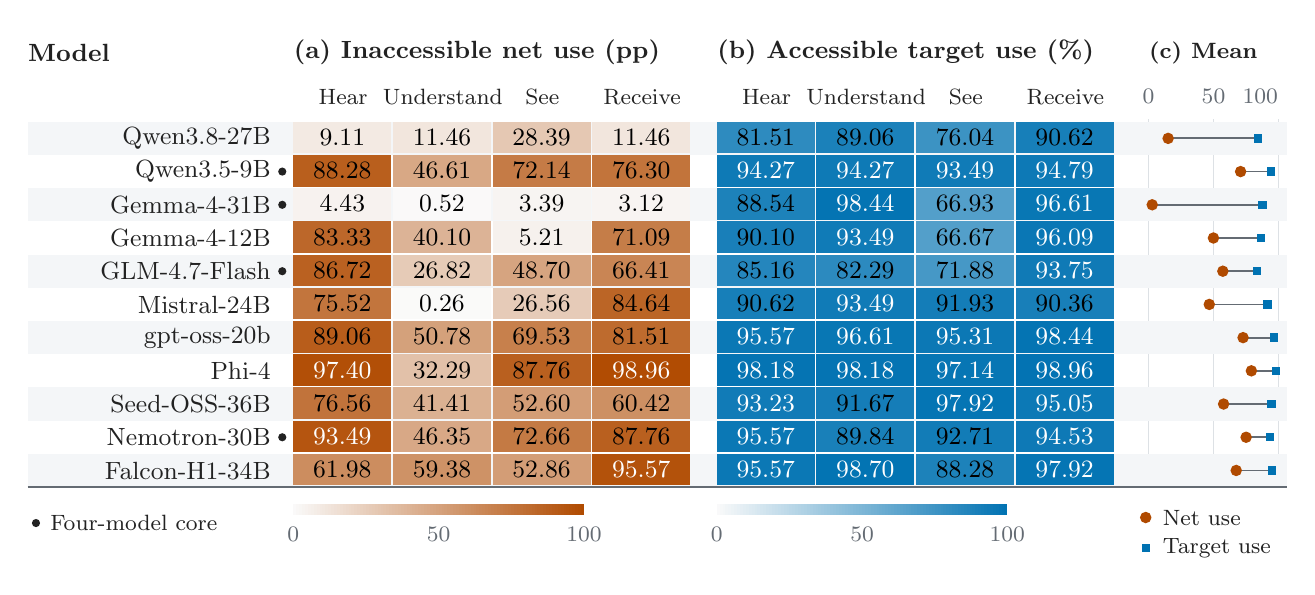
\begin{tikzpicture}[x=1pt,y=-1pt]
\path[use as bounding box] (0,0) rectangle (455,195);
\node[anchor=west,inner sep=0pt,text={rgb,255:red,34;green,34;blue,34},font=\fontsize{9}{10}\selectfont\bfseries] at (0.0000,9.0000) {Model};
\node[anchor=west,inner sep=0pt,text={rgb,255:red,34;green,34;blue,34},font=\fontsize{9}{10}\selectfont\bfseries] at (96.0000,9.0000) {(a) Inaccessible net use (pp)};
\node[anchor=west,inner sep=0pt,text={rgb,255:red,34;green,34;blue,34},font=\fontsize{9}{10}\selectfont\bfseries] at (249.0000,9.0000) {(b) Accessible target use (\%)};
\node[anchor=west,inner sep=0pt,text={rgb,255:red,34;green,34;blue,34},font=\fontsize{8.5}{9.5}\selectfont\bfseries] at (405.0000,9.0000) {(c) Mean};
\node[anchor=center,inner sep=0pt,text={rgb,255:red,34;green,34;blue,34},font=\fontsize{8.3}{9.3}\selectfont] at (114.0000,25.0000) {Hear};
\node[anchor=center,inner sep=0pt,text={rgb,255:red,34;green,34;blue,34},font=\fontsize{8.3}{9.3}\selectfont] at (267.0000,25.0000) {Hear};
\node[anchor=center,inner sep=0pt,text={rgb,255:red,34;green,34;blue,34},font=\fontsize{8.3}{9.3}\selectfont] at (150.0000,25.0000) {Understand};
\node[anchor=center,inner sep=0pt,text={rgb,255:red,34;green,34;blue,34},font=\fontsize{8.3}{9.3}\selectfont] at (303.0000,25.0000) {Understand};
\node[anchor=center,inner sep=0pt,text={rgb,255:red,34;green,34;blue,34},font=\fontsize{8.3}{9.3}\selectfont] at (186.0000,25.0000) {See};
\node[anchor=center,inner sep=0pt,text={rgb,255:red,34;green,34;blue,34},font=\fontsize{8.3}{9.3}\selectfont] at (339.0000,25.0000) {See};
\node[anchor=center,inner sep=0pt,text={rgb,255:red,34;green,34;blue,34},font=\fontsize{8.3}{9.3}\selectfont] at (222.0000,25.0000) {Receive};
\node[anchor=center,inner sep=0pt,text={rgb,255:red,34;green,34;blue,34},font=\fontsize{8.3}{9.3}\selectfont] at (375.0000,25.0000) {Receive};
\draw[draw={rgb,255:red,221;green,225;blue,229},line width=0.4pt] (405.0000,33.0000)--(405.0000,165.0000);
\node[anchor=center,inner sep=0pt,text={rgb,255:red,100;green,107;blue,115},font=\fontsize{8}{9}\selectfont] at (405.0000,25.0000) {0};
\draw[draw={rgb,255:red,221;green,225;blue,229},line width=0.4pt] (428.5000,33.0000)--(428.5000,165.0000);
\node[anchor=center,inner sep=0pt,text={rgb,255:red,100;green,107;blue,115},font=\fontsize{8}{9}\selectfont] at (428.5000,25.0000) {50};
\draw[draw={rgb,255:red,221;green,225;blue,229},line width=0.4pt] (452.0000,33.0000)--(452.0000,165.0000);
\node[anchor=east,inner sep=0pt,text={rgb,255:red,100;green,107;blue,115},font=\fontsize{8}{9}\selectfont] at (452.0000,25.0000) {100};
\fill[fill={rgb,255:red,244;green,246;blue,248}] (0.0000,34.0000) rectangle (455.0000,46.0000);
\node[anchor=east,inner sep=0pt,text={rgb,255:red,34;green,34;blue,34},font=\fontsize{9}{10}\selectfont] at (88.0000,40.0000) {Qwen3.8-27B};
\fill[fill={rgb,255:red,243;green,234;blue,227}] (96.0000,34.0000) rectangle (131.4000,45.4000);
\node[anchor=center,inner sep=0pt,text={rgb,255:red,0;green,0;blue,0},font=\fontsize{8.8}{9.8}\selectfont] at (113.7000,39.7000) {9.11};
\fill[fill={rgb,255:red,242;green,230;blue,221}] (132.0000,34.0000) rectangle (167.4000,45.4000);
\node[anchor=center,inner sep=0pt,text={rgb,255:red,0;green,0;blue,0},font=\fontsize{8.8}{9.8}\selectfont] at (149.7000,39.7000) {11.46};
\fill[fill={rgb,255:red,229;green,200;blue,179}] (168.0000,34.0000) rectangle (203.4000,45.4000);
\node[anchor=center,inner sep=0pt,text={rgb,255:red,0;green,0;blue,0},font=\fontsize{8.8}{9.8}\selectfont] at (185.7000,39.7000) {28.39};
\fill[fill={rgb,255:red,242;green,230;blue,221}] (204.0000,34.0000) rectangle (239.4000,45.4000);
\node[anchor=center,inner sep=0pt,text={rgb,255:red,0;green,0;blue,0},font=\fontsize{8.8}{9.8}\selectfont] at (221.7000,39.7000) {11.46};
\fill[fill={rgb,255:red,46;green,139;blue,191}] (249.0000,34.0000) rectangle (284.4000,45.4000);
\node[anchor=center,inner sep=0pt,text={rgb,255:red,0;green,0;blue,0},font=\fontsize{8.8}{9.8}\selectfont] at (266.7000,39.7000) {81.51};
\fill[fill={rgb,255:red,27;green,129;blue,186}] (285.0000,34.0000) rectangle (320.4000,45.4000);
\node[anchor=center,inner sep=0pt,text={rgb,255:red,0;green,0;blue,0},font=\fontsize{8.8}{9.8}\selectfont] at (302.7000,39.7000) {89.06};
\fill[fill={rgb,255:red,60;green,147;blue,195}] (321.0000,34.0000) rectangle (356.4000,45.4000);
\node[anchor=center,inner sep=0pt,text={rgb,255:red,0;green,0;blue,0},font=\fontsize{8.8}{9.8}\selectfont] at (338.7000,39.7000) {76.04};
\fill[fill={rgb,255:red,23;green,127;blue,185}] (357.0000,34.0000) rectangle (392.4000,45.4000);
\node[anchor=center,inner sep=0pt,text={rgb,255:red,0;green,0;blue,0},font=\fontsize{8.8}{9.8}\selectfont] at (374.7000,39.7000) {90.62};
\draw[draw={rgb,255:red,100;green,107;blue,115},line width=0.65pt] (412.0990,40.0000)--(444.6257,40.0000);
\draw[draw={rgb,255:red,176;green,74;blue,0},fill={rgb,255:red,176;green,74;blue,0},line width=.7pt] (412.0990,40.0000) circle[radius=1.7pt];
\fill[fill={rgb,255:red,0;green,114;blue,178}] (443.1257,38.5000) rectangle (446.1257,41.5000);
\node[anchor=east,inner sep=0pt,text={rgb,255:red,34;green,34;blue,34},font=\fontsize{9}{10}\selectfont] at (88.0000,52.0000) {Qwen3.5-9B};
\draw[draw={rgb,255:red,34;green,34;blue,34},fill={rgb,255:red,34;green,34;blue,34},line width=.7pt] (92.0000,52.0000) circle[radius=1.1pt];
\fill[fill={rgb,255:red,185;green,95;blue,29}] (96.0000,46.0000) rectangle (131.4000,57.4000);
\node[anchor=center,inner sep=0pt,text={rgb,255:red,0;green,0;blue,0},font=\fontsize{8.8}{9.8}\selectfont] at (113.7000,51.7000) {88.28};
\fill[fill={rgb,255:red,216;green,168;blue,133}] (132.0000,46.0000) rectangle (167.4000,57.4000);
\node[anchor=center,inner sep=0pt,text={rgb,255:red,0;green,0;blue,0},font=\fontsize{8.8}{9.8}\selectfont] at (149.7000,51.7000) {46.61};
\fill[fill={rgb,255:red,197;green,123;blue,70}] (168.0000,46.0000) rectangle (203.4000,57.4000);
\node[anchor=center,inner sep=0pt,text={rgb,255:red,0;green,0;blue,0},font=\fontsize{8.8}{9.8}\selectfont] at (185.7000,51.7000) {72.14};
\fill[fill={rgb,255:red,194;green,116;blue,59}] (204.0000,46.0000) rectangle (239.4000,57.4000);
\node[anchor=center,inner sep=0pt,text={rgb,255:red,0;green,0;blue,0},font=\fontsize{8.8}{9.8}\selectfont] at (221.7000,51.7000) {76.30};
\fill[fill={rgb,255:red,14;green,122;blue,182}] (249.0000,46.0000) rectangle (284.4000,57.4000);
\node[anchor=center,inner sep=0pt,text={rgb,255:red,255;green,255;blue,255},font=\fontsize{8.8}{9.8}\selectfont] at (266.7000,51.7000) {94.27};
\fill[fill={rgb,255:red,14;green,122;blue,182}] (285.0000,46.0000) rectangle (320.4000,57.4000);
\node[anchor=center,inner sep=0pt,text={rgb,255:red,255;green,255;blue,255},font=\fontsize{8.8}{9.8}\selectfont] at (302.7000,51.7000) {94.27};
\fill[fill={rgb,255:red,16;green,123;blue,183}] (321.0000,46.0000) rectangle (356.4000,57.4000);
\node[anchor=center,inner sep=0pt,text={rgb,255:red,255;green,255;blue,255},font=\fontsize{8.8}{9.8}\selectfont] at (338.7000,51.7000) {93.49};
\fill[fill={rgb,255:red,13;green,121;blue,182}] (357.0000,46.0000) rectangle (392.4000,57.4000);
\node[anchor=center,inner sep=0pt,text={rgb,255:red,255;green,255;blue,255},font=\fontsize{8.8}{9.8}\selectfont] at (374.7000,51.7000) {94.79};
\draw[draw={rgb,255:red,100;green,107;blue,115},line width=0.65pt] (438.2917,52.0000)--(449.2767,52.0000);
\draw[draw={rgb,255:red,176;green,74;blue,0},fill={rgb,255:red,176;green,74;blue,0},line width=.7pt] (438.2917,52.0000) circle[radius=1.7pt];
\fill[fill={rgb,255:red,0;green,114;blue,178}] (447.7767,50.5000) rectangle (450.7767,53.5000);
\fill[fill={rgb,255:red,244;green,246;blue,248}] (0.0000,58.0000) rectangle (455.0000,70.0000);
\node[anchor=east,inner sep=0pt,text={rgb,255:red,34;green,34;blue,34},font=\fontsize{9}{10}\selectfont] at (88.0000,64.0000) {Gemma-4-31B};
\draw[draw={rgb,255:red,34;green,34;blue,34},fill={rgb,255:red,34;green,34;blue,34},line width=.7pt] (92.0000,64.0000) circle[radius=1.1pt];
\fill[fill={rgb,255:red,247;green,242;blue,239}] (96.0000,58.0000) rectangle (131.4000,69.4000);
\node[anchor=center,inner sep=0pt,text={rgb,255:red,0;green,0;blue,0},font=\fontsize{8.8}{9.8}\selectfont] at (113.7000,63.7000) {4.43};
\fill[fill={rgb,255:red,250;green,249;blue,249}] (132.0000,58.0000) rectangle (167.4000,69.4000);
\node[anchor=center,inner sep=0pt,text={rgb,255:red,0;green,0;blue,0},font=\fontsize{8.8}{9.8}\selectfont] at (149.7000,63.7000) {0.52};
\fill[fill={rgb,255:red,247;green,244;blue,242}] (168.0000,58.0000) rectangle (203.4000,69.4000);
\node[anchor=center,inner sep=0pt,text={rgb,255:red,0;green,0;blue,0},font=\fontsize{8.8}{9.8}\selectfont] at (185.7000,63.7000) {3.39};
\fill[fill={rgb,255:red,248;green,244;blue,242}] (204.0000,58.0000) rectangle (239.4000,69.4000);
\node[anchor=center,inner sep=0pt,text={rgb,255:red,0;green,0;blue,0},font=\fontsize{8.8}{9.8}\selectfont] at (221.7000,63.7000) {3.12};
\fill[fill={rgb,255:red,29;green,130;blue,186}] (249.0000,58.0000) rectangle (284.4000,69.4000);
\node[anchor=center,inner sep=0pt,text={rgb,255:red,0;green,0;blue,0},font=\fontsize{8.8}{9.8}\selectfont] at (266.7000,63.7000) {88.54};
\fill[fill={rgb,255:red,4;green,116;blue,179}] (285.0000,58.0000) rectangle (320.4000,69.4000);
\node[anchor=center,inner sep=0pt,text={rgb,255:red,255;green,255;blue,255},font=\fontsize{8.8}{9.8}\selectfont] at (302.7000,63.7000) {98.44};
\fill[fill={rgb,255:red,83;green,159;blue,202}] (321.0000,58.0000) rectangle (356.4000,69.4000);
\node[anchor=center,inner sep=0pt,text={rgb,255:red,0;green,0;blue,0},font=\fontsize{8.8}{9.8}\selectfont] at (338.7000,63.7000) {66.93};
\fill[fill={rgb,255:red,8;green,119;blue,180}] (357.0000,58.0000) rectangle (392.4000,69.4000);
\node[anchor=center,inner sep=0pt,text={rgb,255:red,255;green,255;blue,255},font=\fontsize{8.8}{9.8}\selectfont] at (374.7000,63.7000) {96.61};
\draw[draw={rgb,255:red,100;green,107;blue,115},line width=0.65pt] (406.3464,64.0000)--(446.1862,64.0000);
\draw[draw={rgb,255:red,176;green,74;blue,0},fill={rgb,255:red,176;green,74;blue,0},line width=.7pt] (406.3464,64.0000) circle[radius=1.7pt];
\fill[fill={rgb,255:red,0;green,114;blue,178}] (444.6862,62.5000) rectangle (447.6862,65.5000);
\node[anchor=east,inner sep=0pt,text={rgb,255:red,34;green,34;blue,34},font=\fontsize{9}{10}\selectfont] at (88.0000,76.0000) {Gemma-4-12B};
\fill[fill={rgb,255:red,188;green,103;blue,42}] (96.0000,70.0000) rectangle (131.4000,81.4000);
\node[anchor=center,inner sep=0pt,text={rgb,255:red,0;green,0;blue,0},font=\fontsize{8.8}{9.8}\selectfont] at (113.7000,75.7000) {83.33};
\fill[fill={rgb,255:red,220;green,179;blue,150}] (132.0000,70.0000) rectangle (167.4000,81.4000);
\node[anchor=center,inner sep=0pt,text={rgb,255:red,0;green,0;blue,0},font=\fontsize{8.8}{9.8}\selectfont] at (149.7000,75.7000) {40.10};
\fill[fill={rgb,255:red,246;green,241;blue,237}] (168.0000,70.0000) rectangle (203.4000,81.4000);
\node[anchor=center,inner sep=0pt,text={rgb,255:red,0;green,0;blue,0},font=\fontsize{8.8}{9.8}\selectfont] at (185.7000,75.7000) {5.21};
\fill[fill={rgb,255:red,197;green,125;blue,72}] (204.0000,70.0000) rectangle (239.4000,81.4000);
\node[anchor=center,inner sep=0pt,text={rgb,255:red,0;green,0;blue,0},font=\fontsize{8.8}{9.8}\selectfont] at (221.7000,75.7000) {71.09};
\fill[fill={rgb,255:red,25;green,127;blue,185}] (249.0000,70.0000) rectangle (284.4000,81.4000);
\node[anchor=center,inner sep=0pt,text={rgb,255:red,0;green,0;blue,0},font=\fontsize{8.8}{9.8}\selectfont] at (266.7000,75.7000) {90.10};
\fill[fill={rgb,255:red,16;green,123;blue,183}] (285.0000,70.0000) rectangle (320.4000,81.4000);
\node[anchor=center,inner sep=0pt,text={rgb,255:red,255;green,255;blue,255},font=\fontsize{8.8}{9.8}\selectfont] at (302.7000,75.7000) {93.49};
\fill[fill={rgb,255:red,83;green,159;blue,202}] (321.0000,70.0000) rectangle (356.4000,81.4000);
\node[anchor=center,inner sep=0pt,text={rgb,255:red,0;green,0;blue,0},font=\fontsize{8.8}{9.8}\selectfont] at (338.7000,75.7000) {66.67};
\fill[fill={rgb,255:red,10;green,119;blue,181}] (357.0000,70.0000) rectangle (392.4000,81.4000);
\node[anchor=center,inner sep=0pt,text={rgb,255:red,255;green,255;blue,255},font=\fontsize{8.8}{9.8}\selectfont] at (374.7000,75.7000) {96.09};
\draw[draw={rgb,255:red,100;green,107;blue,115},line width=0.65pt] (428.4694,76.0000)--(445.6966,76.0000);
\draw[draw={rgb,255:red,176;green,74;blue,0},fill={rgb,255:red,176;green,74;blue,0},line width=.7pt] (428.4694,76.0000) circle[radius=1.7pt];
\fill[fill={rgb,255:red,0;green,114;blue,178}] (444.1966,74.5000) rectangle (447.1966,77.5000);
\fill[fill={rgb,255:red,244;green,246;blue,248}] (0.0000,82.0000) rectangle (455.0000,94.0000);
\node[anchor=east,inner sep=0pt,text={rgb,255:red,34;green,34;blue,34},font=\fontsize{9}{10}\selectfont] at (88.0000,88.0000) {GLM-4.7-Flash};
\draw[draw={rgb,255:red,34;green,34;blue,34},fill={rgb,255:red,34;green,34;blue,34},line width=.7pt] (92.0000,88.0000) circle[radius=1.1pt];
\fill[fill={rgb,255:red,186;green,97;blue,33}] (96.0000,82.0000) rectangle (131.4000,93.4000);
\node[anchor=center,inner sep=0pt,text={rgb,255:red,0;green,0;blue,0},font=\fontsize{8.8}{9.8}\selectfont] at (113.7000,87.7000) {86.72};
\fill[fill={rgb,255:red,230;green,203;blue,183}] (132.0000,82.0000) rectangle (167.4000,93.4000);
\node[anchor=center,inner sep=0pt,text={rgb,255:red,0;green,0;blue,0},font=\fontsize{8.8}{9.8}\selectfont] at (149.7000,87.7000) {26.82};
\fill[fill={rgb,255:red,214;green,164;blue,128}] (168.0000,82.0000) rectangle (203.4000,93.4000);
\node[anchor=center,inner sep=0pt,text={rgb,255:red,0;green,0;blue,0},font=\fontsize{8.8}{9.8}\selectfont] at (185.7000,87.7000) {48.70};
\fill[fill={rgb,255:red,201;green,133;blue,84}] (204.0000,82.0000) rectangle (239.4000,93.4000);
\node[anchor=center,inner sep=0pt,text={rgb,255:red,0;green,0;blue,0},font=\fontsize{8.8}{9.8}\selectfont] at (221.7000,87.7000) {66.41};
\fill[fill={rgb,255:red,37;green,134;blue,189}] (249.0000,82.0000) rectangle (284.4000,93.4000);
\node[anchor=center,inner sep=0pt,text={rgb,255:red,0;green,0;blue,0},font=\fontsize{8.8}{9.8}\selectfont] at (266.7000,87.7000) {85.16};
\fill[fill={rgb,255:red,44;green,138;blue,191}] (285.0000,82.0000) rectangle (320.4000,93.4000);
\node[anchor=center,inner sep=0pt,text={rgb,255:red,0;green,0;blue,0},font=\fontsize{8.8}{9.8}\selectfont] at (302.7000,87.7000) {82.29};
\fill[fill={rgb,255:red,70;green,152;blue,198}] (321.0000,82.0000) rectangle (356.4000,93.4000);
\node[anchor=center,inner sep=0pt,text={rgb,255:red,0;green,0;blue,0},font=\fontsize{8.8}{9.8}\selectfont] at (338.7000,87.7000) {71.88};
\fill[fill={rgb,255:red,16;green,122;blue,182}] (357.0000,82.0000) rectangle (392.4000,93.4000);
\node[anchor=center,inner sep=0pt,text={rgb,255:red,255;green,255;blue,255},font=\fontsize{8.8}{9.8}\selectfont] at (374.7000,87.7000) {93.75};
\draw[draw={rgb,255:red,100;green,107;blue,115},line width=0.65pt] (431.8659,88.0000)--(444.1361,88.0000);
\draw[draw={rgb,255:red,176;green,74;blue,0},fill={rgb,255:red,176;green,74;blue,0},line width=.7pt] (431.8659,88.0000) circle[radius=1.7pt];
\fill[fill={rgb,255:red,0;green,114;blue,178}] (442.6361,86.5000) rectangle (445.6361,89.5000);
\node[anchor=east,inner sep=0pt,text={rgb,255:red,34;green,34;blue,34},font=\fontsize{9}{10}\selectfont] at (88.0000,100.0000) {Mistral-24B};
\fill[fill={rgb,255:red,194;green,117;blue,61}] (96.0000,94.0000) rectangle (131.4000,105.4000);
\node[anchor=center,inner sep=0pt,text={rgb,255:red,0;green,0;blue,0},font=\fontsize{8.8}{9.8}\selectfont] at (113.7000,99.7000) {75.52};
\fill[fill={rgb,255:red,250;green,250;blue,249}] (132.0000,94.0000) rectangle (167.4000,105.4000);
\node[anchor=center,inner sep=0pt,text={rgb,255:red,0;green,0;blue,0},font=\fontsize{8.8}{9.8}\selectfont] at (149.7000,99.7000) {0.26};
\fill[fill={rgb,255:red,230;green,203;blue,184}] (168.0000,94.0000) rectangle (203.4000,105.4000);
\node[anchor=center,inner sep=0pt,text={rgb,255:red,0;green,0;blue,0},font=\fontsize{8.8}{9.8}\selectfont] at (185.7000,99.7000) {26.56};
\fill[fill={rgb,255:red,187;green,101;blue,38}] (204.0000,94.0000) rectangle (239.4000,105.4000);
\node[anchor=center,inner sep=0pt,text={rgb,255:red,0;green,0;blue,0},font=\fontsize{8.8}{9.8}\selectfont] at (221.7000,99.7000) {84.64};
\fill[fill={rgb,255:red,23;green,127;blue,185}] (249.0000,94.0000) rectangle (284.4000,105.4000);
\node[anchor=center,inner sep=0pt,text={rgb,255:red,0;green,0;blue,0},font=\fontsize{8.8}{9.8}\selectfont] at (266.7000,99.7000) {90.62};
\fill[fill={rgb,255:red,16;green,123;blue,183}] (285.0000,94.0000) rectangle (320.4000,105.4000);
\node[anchor=center,inner sep=0pt,text={rgb,255:red,255;green,255;blue,255},font=\fontsize{8.8}{9.8}\selectfont] at (302.7000,99.7000) {93.49};
\fill[fill={rgb,255:red,20;green,125;blue,184}] (321.0000,94.0000) rectangle (356.4000,105.4000);
\node[anchor=center,inner sep=0pt,text={rgb,255:red,0;green,0;blue,0},font=\fontsize{8.8}{9.8}\selectfont] at (338.7000,99.7000) {91.93};
\fill[fill={rgb,255:red,24;green,127;blue,185}] (357.0000,94.0000) rectangle (392.4000,105.4000);
\node[anchor=center,inner sep=0pt,text={rgb,255:red,0;green,0;blue,0},font=\fontsize{8.8}{9.8}\selectfont] at (374.7000,99.7000) {90.36};
\draw[draw={rgb,255:red,100;green,107;blue,115},line width=0.65pt] (426.9701,100.0000)--(448.0527,100.0000);
\draw[draw={rgb,255:red,176;green,74;blue,0},fill={rgb,255:red,176;green,74;blue,0},line width=.7pt] (426.9701,100.0000) circle[radius=1.7pt];
\fill[fill={rgb,255:red,0;green,114;blue,178}] (446.5527,98.5000) rectangle (449.5527,101.5000);
\fill[fill={rgb,255:red,244;green,246;blue,248}] (0.0000,106.0000) rectangle (455.0000,118.0000);
\node[anchor=east,inner sep=0pt,text={rgb,255:red,34;green,34;blue,34},font=\fontsize{9}{10}\selectfont] at (88.0000,112.0000) {gpt-oss-20b};
\fill[fill={rgb,255:red,184;green,93;blue,27}] (96.0000,106.0000) rectangle (131.4000,117.4000);
\node[anchor=center,inner sep=0pt,text={rgb,255:red,0;green,0;blue,0},font=\fontsize{8.8}{9.8}\selectfont] at (113.7000,111.7000) {89.06};
\fill[fill={rgb,255:red,212;green,161;blue,123}] (132.0000,106.0000) rectangle (167.4000,117.4000);
\node[anchor=center,inner sep=0pt,text={rgb,255:red,0;green,0;blue,0},font=\fontsize{8.8}{9.8}\selectfont] at (149.7000,111.7000) {50.78};
\fill[fill={rgb,255:red,199;green,128;blue,76}] (168.0000,106.0000) rectangle (203.4000,117.4000);
\node[anchor=center,inner sep=0pt,text={rgb,255:red,0;green,0;blue,0},font=\fontsize{8.8}{9.8}\selectfont] at (185.7000,111.7000) {69.53};
\fill[fill={rgb,255:red,190;green,107;blue,46}] (204.0000,106.0000) rectangle (239.4000,117.4000);
\node[anchor=center,inner sep=0pt,text={rgb,255:red,0;green,0;blue,0},font=\fontsize{8.8}{9.8}\selectfont] at (221.7000,111.7000) {81.51};
\fill[fill={rgb,255:red,11;green,120;blue,181}] (249.0000,106.0000) rectangle (284.4000,117.4000);
\node[anchor=center,inner sep=0pt,text={rgb,255:red,255;green,255;blue,255},font=\fontsize{8.8}{9.8}\selectfont] at (266.7000,111.7000) {95.57};
\fill[fill={rgb,255:red,8;green,119;blue,180}] (285.0000,106.0000) rectangle (320.4000,117.4000);
\node[anchor=center,inner sep=0pt,text={rgb,255:red,255;green,255;blue,255},font=\fontsize{8.8}{9.8}\selectfont] at (302.7000,111.7000) {96.61};
\fill[fill={rgb,255:red,12;green,120;blue,181}] (321.0000,106.0000) rectangle (356.4000,117.4000);
\node[anchor=center,inner sep=0pt,text={rgb,255:red,255;green,255;blue,255},font=\fontsize{8.8}{9.8}\selectfont] at (338.7000,111.7000) {95.31};
\fill[fill={rgb,255:red,4;green,116;blue,179}] (357.0000,106.0000) rectangle (392.4000,117.4000);
\node[anchor=center,inner sep=0pt,text={rgb,255:red,255;green,255;blue,255},font=\fontsize{8.8}{9.8}\selectfont] at (374.7000,111.7000) {98.44};
\draw[draw={rgb,255:red,100;green,107;blue,115},line width=0.65pt] (439.1790,112.0000)--(450.3477,112.0000);
\draw[draw={rgb,255:red,176;green,74;blue,0},fill={rgb,255:red,176;green,74;blue,0},line width=.7pt] (439.1790,112.0000) circle[radius=1.7pt];
\fill[fill={rgb,255:red,0;green,114;blue,178}] (448.8477,110.5000) rectangle (451.8477,113.5000);
\node[anchor=east,inner sep=0pt,text={rgb,255:red,34;green,34;blue,34},font=\fontsize{9}{10}\selectfont] at (88.0000,124.0000) {Phi-4};
\fill[fill={rgb,255:red,178;green,79;blue,7}] (96.0000,118.0000) rectangle (131.4000,129.4000);
\node[anchor=center,inner sep=0pt,text={rgb,255:red,255;green,255;blue,255},font=\fontsize{8.8}{9.8}\selectfont] at (113.7000,123.7000) {97.40};
\fill[fill={rgb,255:red,226;green,193;blue,169}] (132.0000,118.0000) rectangle (167.4000,129.4000);
\node[anchor=center,inner sep=0pt,text={rgb,255:red,0;green,0;blue,0},font=\fontsize{8.8}{9.8}\selectfont] at (149.7000,123.7000) {32.29};
\fill[fill={rgb,255:red,185;green,96;blue,31}] (168.0000,118.0000) rectangle (203.4000,129.4000);
\node[anchor=center,inner sep=0pt,text={rgb,255:red,0;green,0;blue,0},font=\fontsize{8.8}{9.8}\selectfont] at (185.7000,123.7000) {87.76};
\fill[fill={rgb,255:red,177;green,76;blue,3}] (204.0000,118.0000) rectangle (239.4000,129.4000);
\node[anchor=center,inner sep=0pt,text={rgb,255:red,255;green,255;blue,255},font=\fontsize{8.8}{9.8}\selectfont] at (221.7000,123.7000) {98.96};
\fill[fill={rgb,255:red,5;green,116;blue,179}] (249.0000,118.0000) rectangle (284.4000,129.4000);
\node[anchor=center,inner sep=0pt,text={rgb,255:red,255;green,255;blue,255},font=\fontsize{8.8}{9.8}\selectfont] at (266.7000,123.7000) {98.18};
\fill[fill={rgb,255:red,5;green,116;blue,179}] (285.0000,118.0000) rectangle (320.4000,129.4000);
\node[anchor=center,inner sep=0pt,text={rgb,255:red,255;green,255;blue,255},font=\fontsize{8.8}{9.8}\selectfont] at (302.7000,123.7000) {98.18};
\fill[fill={rgb,255:red,7;green,118;blue,180}] (321.0000,118.0000) rectangle (356.4000,129.4000);
\node[anchor=center,inner sep=0pt,text={rgb,255:red,255;green,255;blue,255},font=\fontsize{8.8}{9.8}\selectfont] at (338.7000,123.7000) {97.14};
\fill[fill={rgb,255:red,3;green,115;blue,179}] (357.0000,118.0000) rectangle (392.4000,129.4000);
\node[anchor=center,inner sep=0pt,text={rgb,255:red,255;green,255;blue,255},font=\fontsize{8.8}{9.8}\selectfont] at (374.7000,123.7000) {98.96};
\draw[draw={rgb,255:red,100;green,107;blue,115},line width=0.65pt] (442.1777,124.0000)--(451.1126,124.0000);
\draw[draw={rgb,255:red,176;green,74;blue,0},fill={rgb,255:red,176;green,74;blue,0},line width=.7pt] (442.1777,124.0000) circle[radius=1.7pt];
\fill[fill={rgb,255:red,0;green,114;blue,178}] (449.6126,122.5000) rectangle (452.6126,125.5000);
\fill[fill={rgb,255:red,244;green,246;blue,248}] (0.0000,130.0000) rectangle (455.0000,142.0000);
\node[anchor=east,inner sep=0pt,text={rgb,255:red,34;green,34;blue,34},font=\fontsize{9}{10}\selectfont] at (88.0000,136.0000) {Seed-OSS-36B};
\fill[fill={rgb,255:red,193;green,115;blue,59}] (96.0000,130.0000) rectangle (131.4000,141.4000);
\node[anchor=center,inner sep=0pt,text={rgb,255:red,0;green,0;blue,0},font=\fontsize{8.8}{9.8}\selectfont] at (113.7000,135.7000) {76.56};
\fill[fill={rgb,255:red,219;green,177;blue,146}] (132.0000,130.0000) rectangle (167.4000,141.4000);
\node[anchor=center,inner sep=0pt,text={rgb,255:red,0;green,0;blue,0},font=\fontsize{8.8}{9.8}\selectfont] at (149.7000,135.7000) {41.41};
\fill[fill={rgb,255:red,211;green,157;blue,118}] (168.0000,130.0000) rectangle (203.4000,141.4000);
\node[anchor=center,inner sep=0pt,text={rgb,255:red,0;green,0;blue,0},font=\fontsize{8.8}{9.8}\selectfont] at (185.7000,135.7000) {52.60};
\fill[fill={rgb,255:red,205;green,144;blue,99}] (204.0000,130.0000) rectangle (239.4000,141.4000);
\node[anchor=center,inner sep=0pt,text={rgb,255:red,0;green,0;blue,0},font=\fontsize{8.8}{9.8}\selectfont] at (221.7000,135.7000) {60.42};
\fill[fill={rgb,255:red,17;green,123;blue,183}] (249.0000,130.0000) rectangle (284.4000,141.4000);
\node[anchor=center,inner sep=0pt,text={rgb,255:red,255;green,255;blue,255},font=\fontsize{8.8}{9.8}\selectfont] at (266.7000,135.7000) {93.23};
\fill[fill={rgb,255:red,21;green,125;blue,184}] (285.0000,130.0000) rectangle (320.4000,141.4000);
\node[anchor=center,inner sep=0pt,text={rgb,255:red,0;green,0;blue,0},font=\fontsize{8.8}{9.8}\selectfont] at (302.7000,135.7000) {91.67};
\fill[fill={rgb,255:red,5;green,117;blue,180}] (321.0000,130.0000) rectangle (356.4000,141.4000);
\node[anchor=center,inner sep=0pt,text={rgb,255:red,255;green,255;blue,255},font=\fontsize{8.8}{9.8}\selectfont] at (338.7000,135.7000) {97.92};
\fill[fill={rgb,255:red,12;green,121;blue,182}] (357.0000,130.0000) rectangle (392.4000,141.4000);
\node[anchor=center,inner sep=0pt,text={rgb,255:red,255;green,255;blue,255},font=\fontsize{8.8}{9.8}\selectfont] at (374.7000,135.7000) {95.05};
\draw[draw={rgb,255:red,100;green,107;blue,115},line width=0.65pt] (432.1413,136.0000)--(449.3991,136.0000);
\draw[draw={rgb,255:red,176;green,74;blue,0},fill={rgb,255:red,176;green,74;blue,0},line width=.7pt] (432.1413,136.0000) circle[radius=1.7pt];
\fill[fill={rgb,255:red,0;green,114;blue,178}] (447.8991,134.5000) rectangle (450.8991,137.5000);
\node[anchor=east,inner sep=0pt,text={rgb,255:red,34;green,34;blue,34},font=\fontsize{9}{10}\selectfont] at (88.0000,148.0000) {Nemotron-30B};
\draw[draw={rgb,255:red,34;green,34;blue,34},fill={rgb,255:red,34;green,34;blue,34},line width=.7pt] (92.0000,148.0000) circle[radius=1.1pt];
\fill[fill={rgb,255:red,181;green,85;blue,16}] (96.0000,142.0000) rectangle (131.4000,153.4000);
\node[anchor=center,inner sep=0pt,text={rgb,255:red,255;green,255;blue,255},font=\fontsize{8.8}{9.8}\selectfont] at (113.7000,147.7000) {93.49};
\fill[fill={rgb,255:red,216;green,168;blue,134}] (132.0000,142.0000) rectangle (167.4000,153.4000);
\node[anchor=center,inner sep=0pt,text={rgb,255:red,0;green,0;blue,0},font=\fontsize{8.8}{9.8}\selectfont] at (149.7000,147.7000) {46.35};
\fill[fill={rgb,255:red,196;green,122;blue,68}] (168.0000,142.0000) rectangle (203.4000,153.4000);
\node[anchor=center,inner sep=0pt,text={rgb,255:red,0;green,0;blue,0},font=\fontsize{8.8}{9.8}\selectfont] at (185.7000,147.7000) {72.66};
\fill[fill={rgb,255:red,185;green,96;blue,31}] (204.0000,142.0000) rectangle (239.4000,153.4000);
\node[anchor=center,inner sep=0pt,text={rgb,255:red,0;green,0;blue,0},font=\fontsize{8.8}{9.8}\selectfont] at (221.7000,147.7000) {87.76};
\fill[fill={rgb,255:red,11;green,120;blue,181}] (249.0000,142.0000) rectangle (284.4000,153.4000);
\node[anchor=center,inner sep=0pt,text={rgb,255:red,255;green,255;blue,255},font=\fontsize{8.8}{9.8}\selectfont] at (266.7000,147.7000) {95.57};
\fill[fill={rgb,255:red,25;green,128;blue,185}] (285.0000,142.0000) rectangle (320.4000,153.4000);
\node[anchor=center,inner sep=0pt,text={rgb,255:red,0;green,0;blue,0},font=\fontsize{8.8}{9.8}\selectfont] at (302.7000,147.7000) {89.84};
\fill[fill={rgb,255:red,18;green,124;blue,183}] (321.0000,142.0000) rectangle (356.4000,153.4000);
\node[anchor=center,inner sep=0pt,text={rgb,255:red,0;green,0;blue,0},font=\fontsize{8.8}{9.8}\selectfont] at (338.7000,147.7000) {92.71};
\fill[fill={rgb,255:red,14;green,121;blue,182}] (357.0000,142.0000) rectangle (392.4000,153.4000);
\node[anchor=center,inner sep=0pt,text={rgb,255:red,255;green,255;blue,255},font=\fontsize{8.8}{9.8}\selectfont] at (374.7000,147.7000) {94.53};
\draw[draw={rgb,255:red,100;green,107;blue,115},line width=0.65pt] (440.2806,148.0000)--(448.7871,148.0000);
\draw[draw={rgb,255:red,176;green,74;blue,0},fill={rgb,255:red,176;green,74;blue,0},line width=.7pt] (440.2806,148.0000) circle[radius=1.7pt];
\fill[fill={rgb,255:red,0;green,114;blue,178}] (447.2871,146.5000) rectangle (450.2871,149.5000);
\fill[fill={rgb,255:red,244;green,246;blue,248}] (0.0000,154.0000) rectangle (455.0000,166.0000);
\node[anchor=east,inner sep=0pt,text={rgb,255:red,34;green,34;blue,34},font=\fontsize{9}{10}\selectfont] at (88.0000,160.0000) {Falcon-H1-34B};
\fill[fill={rgb,255:red,204;green,141;blue,95}] (96.0000,154.0000) rectangle (131.4000,165.4000);
\node[anchor=center,inner sep=0pt,text={rgb,255:red,0;green,0;blue,0},font=\fontsize{8.8}{9.8}\selectfont] at (113.7000,159.7000) {61.98};
\fill[fill={rgb,255:red,206;green,146;blue,102}] (132.0000,154.0000) rectangle (167.4000,165.4000);
\node[anchor=center,inner sep=0pt,text={rgb,255:red,0;green,0;blue,0},font=\fontsize{8.8}{9.8}\selectfont] at (149.7000,159.7000) {59.38};
\fill[fill={rgb,255:red,211;green,157;blue,118}] (168.0000,154.0000) rectangle (203.4000,165.4000);
\node[anchor=center,inner sep=0pt,text={rgb,255:red,0;green,0;blue,0},font=\fontsize{8.8}{9.8}\selectfont] at (185.7000,159.7000) {52.86};
\fill[fill={rgb,255:red,179;green,82;blue,11}] (204.0000,154.0000) rectangle (239.4000,165.4000);
\node[anchor=center,inner sep=0pt,text={rgb,255:red,255;green,255;blue,255},font=\fontsize{8.8}{9.8}\selectfont] at (221.7000,159.7000) {95.57};
\fill[fill={rgb,255:red,11;green,120;blue,181}] (249.0000,154.0000) rectangle (284.4000,165.4000);
\node[anchor=center,inner sep=0pt,text={rgb,255:red,255;green,255;blue,255},font=\fontsize{8.8}{9.8}\selectfont] at (266.7000,159.7000) {95.57};
\fill[fill={rgb,255:red,3;green,116;blue,179}] (285.0000,154.0000) rectangle (320.4000,165.4000);
\node[anchor=center,inner sep=0pt,text={rgb,255:red,255;green,255;blue,255},font=\fontsize{8.8}{9.8}\selectfont] at (302.7000,159.7000) {98.70};
\fill[fill={rgb,255:red,29;green,130;blue,186}] (321.0000,154.0000) rectangle (356.4000,165.4000);
\node[anchor=center,inner sep=0pt,text={rgb,255:red,0;green,0;blue,0},font=\fontsize{8.8}{9.8}\selectfont] at (338.7000,159.7000) {88.28};
\fill[fill={rgb,255:red,5;green,117;blue,180}] (357.0000,154.0000) rectangle (392.4000,165.4000);
\node[anchor=center,inner sep=0pt,text={rgb,255:red,255;green,255;blue,255},font=\fontsize{8.8}{9.8}\selectfont] at (374.7000,159.7000) {97.92};
\draw[draw={rgb,255:red,100;green,107;blue,115},line width=0.65pt] (436.7005,160.0000)--(449.7051,160.0000);
\draw[draw={rgb,255:red,176;green,74;blue,0},fill={rgb,255:red,176;green,74;blue,0},line width=.7pt] (436.7005,160.0000) circle[radius=1.7pt];
\fill[fill={rgb,255:red,0;green,114;blue,178}] (448.2051,158.5000) rectangle (451.2051,161.5000);
\draw[draw={rgb,255:red,100;green,107;blue,115},line width=0.65pt] (0.0000,166.0000)--(455.0000,166.0000);
\fill[fill={rgb,255:red,250;green,249;blue,249}] (96.0000,172.0000) rectangle (97.0700,176.0000);
\fill[fill={rgb,255:red,249;green,247;blue,246}] (97.0500,172.0000) rectangle (98.1200,176.0000);
\fill[fill={rgb,255:red,248;green,246;blue,244}] (98.1000,172.0000) rectangle (99.1700,176.0000);
\fill[fill={rgb,255:red,247;green,244;blue,241}] (99.1500,172.0000) rectangle (100.2200,176.0000);
\fill[fill={rgb,255:red,247;green,242;blue,239}] (100.2000,172.0000) rectangle (101.2700,176.0000);
\fill[fill={rgb,255:red,246;green,240;blue,236}] (101.2500,172.0000) rectangle (102.3200,176.0000);
\fill[fill={rgb,255:red,245;green,239;blue,234}] (102.3000,172.0000) rectangle (103.3700,176.0000);
\fill[fill={rgb,255:red,244;green,237;blue,231}] (103.3500,172.0000) rectangle (104.4200,176.0000);
\fill[fill={rgb,255:red,244;green,235;blue,229}] (104.4000,172.0000) rectangle (105.4700,176.0000);
\fill[fill={rgb,255:red,243;green,233;blue,226}] (105.4500,172.0000) rectangle (106.5200,176.0000);
\fill[fill={rgb,255:red,242;green,232;blue,224}] (106.5000,172.0000) rectangle (107.5700,176.0000);
\fill[fill={rgb,255:red,241;green,230;blue,221}] (107.5500,172.0000) rectangle (108.6200,176.0000);
\fill[fill={rgb,255:red,241;green,228;blue,219}] (108.6000,172.0000) rectangle (109.6700,176.0000);
\fill[fill={rgb,255:red,240;green,226;blue,216}] (109.6500,172.0000) rectangle (110.7200,176.0000);
\fill[fill={rgb,255:red,239;green,224;blue,214}] (110.7000,172.0000) rectangle (111.7700,176.0000);
\fill[fill={rgb,255:red,239;green,223;blue,211}] (111.7500,172.0000) rectangle (112.8200,176.0000);
\fill[fill={rgb,255:red,238;green,221;blue,209}] (112.8000,172.0000) rectangle (113.8700,176.0000);
\fill[fill={rgb,255:red,237;green,219;blue,206}] (113.8500,172.0000) rectangle (114.9200,176.0000);
\fill[fill={rgb,255:red,236;green,217;blue,204}] (114.9000,172.0000) rectangle (115.9700,176.0000);
\fill[fill={rgb,255:red,236;green,216;blue,201}] (115.9500,172.0000) rectangle (117.0200,176.0000);
\fill[fill={rgb,255:red,235;green,214;blue,199}] (117.0000,172.0000) rectangle (118.0700,176.0000);
\fill[fill={rgb,255:red,234;green,212;blue,196}] (118.0500,172.0000) rectangle (119.1200,176.0000);
\fill[fill={rgb,255:red,233;green,210;blue,194}] (119.1000,172.0000) rectangle (120.1700,176.0000);
\fill[fill={rgb,255:red,233;green,209;blue,191}] (120.1500,172.0000) rectangle (121.2200,176.0000);
\fill[fill={rgb,255:red,232;green,207;blue,189}] (121.2000,172.0000) rectangle (122.2700,176.0000);
\fill[fill={rgb,255:red,231;green,205;blue,186}] (122.2500,172.0000) rectangle (123.3200,176.0000);
\fill[fill={rgb,255:red,230;green,203;blue,184}] (123.3000,172.0000) rectangle (124.3700,176.0000);
\fill[fill={rgb,255:red,230;green,202;blue,181}] (124.3500,172.0000) rectangle (125.4200,176.0000);
\fill[fill={rgb,255:red,229;green,200;blue,179}] (125.4000,172.0000) rectangle (126.4700,176.0000);
\fill[fill={rgb,255:red,228;green,198;blue,176}] (126.4500,172.0000) rectangle (127.5200,176.0000);
\fill[fill={rgb,255:red,227;green,196;blue,174}] (127.5000,172.0000) rectangle (128.5700,176.0000);
\fill[fill={rgb,255:red,227;green,195;blue,171}] (128.5500,172.0000) rectangle (129.6200,176.0000);
\fill[fill={rgb,255:red,226;green,193;blue,169}] (129.6000,172.0000) rectangle (130.6700,176.0000);
\fill[fill={rgb,255:red,225;green,191;blue,166}] (130.6500,172.0000) rectangle (131.7200,176.0000);
\fill[fill={rgb,255:red,224;green,189;blue,164}] (131.7000,172.0000) rectangle (132.7700,176.0000);
\fill[fill={rgb,255:red,224;green,188;blue,161}] (132.7500,172.0000) rectangle (133.8200,176.0000);
\fill[fill={rgb,255:red,223;green,186;blue,159}] (133.8000,172.0000) rectangle (134.8700,176.0000);
\fill[fill={rgb,255:red,222;green,184;blue,156}] (134.8500,172.0000) rectangle (135.9200,176.0000);
\fill[fill={rgb,255:red,222;green,182;blue,154}] (135.9000,172.0000) rectangle (136.9700,176.0000);
\fill[fill={rgb,255:red,221;green,180;blue,151}] (136.9500,172.0000) rectangle (138.0200,176.0000);
\fill[fill={rgb,255:red,220;green,179;blue,149}] (138.0000,172.0000) rectangle (139.0700,176.0000);
\fill[fill={rgb,255:red,219;green,177;blue,146}] (139.0500,172.0000) rectangle (140.1200,176.0000);
\fill[fill={rgb,255:red,219;green,175;blue,144}] (140.1000,172.0000) rectangle (141.1700,176.0000);
\fill[fill={rgb,255:red,218;green,173;blue,141}] (141.1500,172.0000) rectangle (142.2200,176.0000);
\fill[fill={rgb,255:red,217;green,172;blue,139}] (142.2000,172.0000) rectangle (143.2700,176.0000);
\fill[fill={rgb,255:red,216;green,170;blue,136}] (143.2500,172.0000) rectangle (144.3200,176.0000);
\fill[fill={rgb,255:red,216;green,168;blue,134}] (144.3000,172.0000) rectangle (145.3700,176.0000);
\fill[fill={rgb,255:red,215;green,166;blue,131}] (145.3500,172.0000) rectangle (146.4200,176.0000);
\fill[fill={rgb,255:red,214;green,165;blue,129}] (146.4000,172.0000) rectangle (147.4700,176.0000);
\fill[fill={rgb,255:red,213;green,163;blue,126}] (147.4500,172.0000) rectangle (148.5200,176.0000);
\fill[fill={rgb,255:red,213;green,161;blue,124}] (148.5000,172.0000) rectangle (149.5700,176.0000);
\fill[fill={rgb,255:red,212;green,159;blue,121}] (149.5500,172.0000) rectangle (150.6200,176.0000);
\fill[fill={rgb,255:red,211;green,158;blue,119}] (150.6000,172.0000) rectangle (151.6700,176.0000);
\fill[fill={rgb,255:red,210;green,156;blue,116}] (151.6500,172.0000) rectangle (152.7200,176.0000);
\fill[fill={rgb,255:red,210;green,154;blue,114}] (152.7000,172.0000) rectangle (153.7700,176.0000);
\fill[fill={rgb,255:red,209;green,152;blue,111}] (153.7500,172.0000) rectangle (154.8200,176.0000);
\fill[fill={rgb,255:red,208;green,151;blue,109}] (154.8000,172.0000) rectangle (155.8700,176.0000);
\fill[fill={rgb,255:red,207;green,149;blue,106}] (155.8500,172.0000) rectangle (156.9200,176.0000);
\fill[fill={rgb,255:red,207;green,147;blue,104}] (156.9000,172.0000) rectangle (157.9700,176.0000);
\fill[fill={rgb,255:red,206;green,145;blue,101}] (157.9500,172.0000) rectangle (159.0200,176.0000);
\fill[fill={rgb,255:red,205;green,144;blue,99}] (159.0000,172.0000) rectangle (160.0700,176.0000);
\fill[fill={rgb,255:red,204;green,142;blue,96}] (160.0500,172.0000) rectangle (161.1200,176.0000);
\fill[fill={rgb,255:red,204;green,140;blue,94}] (161.1000,172.0000) rectangle (162.1700,176.0000);
\fill[fill={rgb,255:red,203;green,138;blue,91}] (162.1500,172.0000) rectangle (163.2200,176.0000);
\fill[fill={rgb,255:red,202;green,136;blue,89}] (163.2000,172.0000) rectangle (164.2700,176.0000);
\fill[fill={rgb,255:red,202;green,135;blue,86}] (164.2500,172.0000) rectangle (165.3200,176.0000);
\fill[fill={rgb,255:red,201;green,133;blue,84}] (165.3000,172.0000) rectangle (166.3700,176.0000);
\fill[fill={rgb,255:red,200;green,131;blue,81}] (166.3500,172.0000) rectangle (167.4200,176.0000);
\fill[fill={rgb,255:red,199;green,129;blue,79}] (167.4000,172.0000) rectangle (168.4700,176.0000);
\fill[fill={rgb,255:red,199;green,128;blue,76}] (168.4500,172.0000) rectangle (169.5200,176.0000);
\fill[fill={rgb,255:red,198;green,126;blue,74}] (169.5000,172.0000) rectangle (170.5700,176.0000);
\fill[fill={rgb,255:red,197;green,124;blue,71}] (170.5500,172.0000) rectangle (171.6200,176.0000);
\fill[fill={rgb,255:red,196;green,122;blue,69}] (171.6000,172.0000) rectangle (172.6700,176.0000);
\fill[fill={rgb,255:red,196;green,121;blue,66}] (172.6500,172.0000) rectangle (173.7200,176.0000);
\fill[fill={rgb,255:red,195;green,119;blue,64}] (173.7000,172.0000) rectangle (174.7700,176.0000);
\fill[fill={rgb,255:red,194;green,117;blue,61}] (174.7500,172.0000) rectangle (175.8200,176.0000);
\fill[fill={rgb,255:red,193;green,115;blue,59}] (175.8000,172.0000) rectangle (176.8700,176.0000);
\fill[fill={rgb,255:red,193;green,114;blue,56}] (176.8500,172.0000) rectangle (177.9200,176.0000);
\fill[fill={rgb,255:red,192;green,112;blue,54}] (177.9000,172.0000) rectangle (178.9700,176.0000);
\fill[fill={rgb,255:red,191;green,110;blue,51}] (178.9500,172.0000) rectangle (180.0200,176.0000);
\fill[fill={rgb,255:red,190;green,108;blue,49}] (180.0000,172.0000) rectangle (181.0700,176.0000);
\fill[fill={rgb,255:red,190;green,107;blue,46}] (181.0500,172.0000) rectangle (182.1200,176.0000);
\fill[fill={rgb,255:red,189;green,105;blue,44}] (182.1000,172.0000) rectangle (183.1700,176.0000);
\fill[fill={rgb,255:red,188;green,103;blue,41}] (183.1500,172.0000) rectangle (184.2200,176.0000);
\fill[fill={rgb,255:red,187;green,101;blue,39}] (184.2000,172.0000) rectangle (185.2700,176.0000);
\fill[fill={rgb,255:red,187;green,100;blue,36}] (185.2500,172.0000) rectangle (186.3200,176.0000);
\fill[fill={rgb,255:red,186;green,98;blue,34}] (186.3000,172.0000) rectangle (187.3700,176.0000);
\fill[fill={rgb,255:red,185;green,96;blue,31}] (187.3500,172.0000) rectangle (188.4200,176.0000);
\fill[fill={rgb,255:red,185;green,94;blue,29}] (188.4000,172.0000) rectangle (189.4700,176.0000);
\fill[fill={rgb,255:red,184;green,92;blue,26}] (189.4500,172.0000) rectangle (190.5200,176.0000);
\fill[fill={rgb,255:red,183;green,91;blue,24}] (190.5000,172.0000) rectangle (191.5700,176.0000);
\fill[fill={rgb,255:red,182;green,89;blue,21}] (191.5500,172.0000) rectangle (192.6200,176.0000);
\fill[fill={rgb,255:red,182;green,87;blue,19}] (192.6000,172.0000) rectangle (193.6700,176.0000);
\fill[fill={rgb,255:red,181;green,85;blue,16}] (193.6500,172.0000) rectangle (194.7200,176.0000);
\fill[fill={rgb,255:red,180;green,84;blue,14}] (194.7000,172.0000) rectangle (195.7700,176.0000);
\fill[fill={rgb,255:red,179;green,82;blue,11}] (195.7500,172.0000) rectangle (196.8200,176.0000);
\fill[fill={rgb,255:red,179;green,80;blue,9}] (196.8000,172.0000) rectangle (197.8700,176.0000);
\fill[fill={rgb,255:red,178;green,78;blue,6}] (197.8500,172.0000) rectangle (198.9200,176.0000);
\fill[fill={rgb,255:red,177;green,77;blue,4}] (198.9000,172.0000) rectangle (199.9700,176.0000);
\fill[fill={rgb,255:red,176;green,75;blue,1}] (199.9500,172.0000) rectangle (201.0200,176.0000);
\node[anchor=center,inner sep=0pt,text={rgb,255:red,100;green,107;blue,115},font=\fontsize{8}{9}\selectfont] at (96.0000,183.0000) {0};
\node[anchor=center,inner sep=0pt,text={rgb,255:red,100;green,107;blue,115},font=\fontsize{8}{9}\selectfont] at (148.5000,183.0000) {50};
\node[anchor=center,inner sep=0pt,text={rgb,255:red,100;green,107;blue,115},font=\fontsize{8}{9}\selectfont] at (201.0000,183.0000) {100};
\fill[fill={rgb,255:red,249;green,249;blue,250}] (249.0000,172.0000) rectangle (250.0700,176.0000);
\fill[fill={rgb,255:red,246;green,248;blue,249}] (250.0500,172.0000) rectangle (251.1200,176.0000);
\fill[fill={rgb,255:red,244;green,247;blue,248}] (251.1000,172.0000) rectangle (252.1700,176.0000);
\fill[fill={rgb,255:red,241;green,245;blue,247}] (252.1500,172.0000) rectangle (253.2200,176.0000);
\fill[fill={rgb,255:red,239;green,244;blue,247}] (253.2000,172.0000) rectangle (254.2700,176.0000);
\fill[fill={rgb,255:red,236;green,243;blue,246}] (254.2500,172.0000) rectangle (255.3200,176.0000);
\fill[fill={rgb,255:red,234;green,241;blue,245}] (255.3000,172.0000) rectangle (256.3700,176.0000);
\fill[fill={rgb,255:red,231;green,240;blue,245}] (256.3500,172.0000) rectangle (257.4200,176.0000);
\fill[fill={rgb,255:red,229;green,238;blue,244}] (257.4000,172.0000) rectangle (258.4700,176.0000);
\fill[fill={rgb,255:red,226;green,237;blue,243}] (258.4500,172.0000) rectangle (259.5200,176.0000);
\fill[fill={rgb,255:red,224;green,236;blue,242}] (259.5000,172.0000) rectangle (260.5700,176.0000);
\fill[fill={rgb,255:red,221;green,234;blue,242}] (260.5500,172.0000) rectangle (261.6200,176.0000);
\fill[fill={rgb,255:red,219;green,233;blue,241}] (261.6000,172.0000) rectangle (262.6700,176.0000);
\fill[fill={rgb,255:red,216;green,232;blue,240}] (262.6500,172.0000) rectangle (263.7200,176.0000);
\fill[fill={rgb,255:red,214;green,230;blue,240}] (263.7000,172.0000) rectangle (264.7700,176.0000);
\fill[fill={rgb,255:red,211;green,229;blue,239}] (264.7500,172.0000) rectangle (265.8200,176.0000);
\fill[fill={rgb,255:red,209;green,228;blue,238}] (265.8000,172.0000) rectangle (266.8700,176.0000);
\fill[fill={rgb,255:red,206;green,226;blue,237}] (266.8500,172.0000) rectangle (267.9200,176.0000);
\fill[fill={rgb,255:red,204;green,225;blue,237}] (267.9000,172.0000) rectangle (268.9700,176.0000);
\fill[fill={rgb,255:red,201;green,223;blue,236}] (268.9500,172.0000) rectangle (270.0200,176.0000);
\fill[fill={rgb,255:red,199;green,222;blue,235}] (270.0000,172.0000) rectangle (271.0700,176.0000);
\fill[fill={rgb,255:red,196;green,221;blue,235}] (271.0500,172.0000) rectangle (272.1200,176.0000);
\fill[fill={rgb,255:red,194;green,219;blue,234}] (272.1000,172.0000) rectangle (273.1700,176.0000);
\fill[fill={rgb,255:red,191;green,218;blue,233}] (273.1500,172.0000) rectangle (274.2200,176.0000);
\fill[fill={rgb,255:red,189;green,217;blue,232}] (274.2000,172.0000) rectangle (275.2700,176.0000);
\fill[fill={rgb,255:red,186;green,215;blue,232}] (275.2500,172.0000) rectangle (276.3200,176.0000);
\fill[fill={rgb,255:red,184;green,214;blue,231}] (276.3000,172.0000) rectangle (277.3700,176.0000);
\fill[fill={rgb,255:red,181;green,213;blue,230}] (277.3500,172.0000) rectangle (278.4200,176.0000);
\fill[fill={rgb,255:red,179;green,211;blue,229}] (278.4000,172.0000) rectangle (279.4700,176.0000);
\fill[fill={rgb,255:red,176;green,210;blue,229}] (279.4500,172.0000) rectangle (280.5200,176.0000);
\fill[fill={rgb,255:red,174;green,209;blue,228}] (280.5000,172.0000) rectangle (281.5700,176.0000);
\fill[fill={rgb,255:red,171;green,207;blue,227}] (281.5500,172.0000) rectangle (282.6200,176.0000);
\fill[fill={rgb,255:red,169;green,206;blue,227}] (282.6000,172.0000) rectangle (283.6700,176.0000);
\fill[fill={rgb,255:red,166;green,204;blue,226}] (283.6500,172.0000) rectangle (284.7200,176.0000);
\fill[fill={rgb,255:red,164;green,203;blue,225}] (284.7000,172.0000) rectangle (285.7700,176.0000);
\fill[fill={rgb,255:red,161;green,202;blue,224}] (285.7500,172.0000) rectangle (286.8200,176.0000);
\fill[fill={rgb,255:red,159;green,200;blue,224}] (286.8000,172.0000) rectangle (287.8700,176.0000);
\fill[fill={rgb,255:red,156;green,199;blue,223}] (287.8500,172.0000) rectangle (288.9200,176.0000);
\fill[fill={rgb,255:red,154;green,198;blue,222}] (288.9000,172.0000) rectangle (289.9700,176.0000);
\fill[fill={rgb,255:red,151;green,196;blue,222}] (289.9500,172.0000) rectangle (291.0200,176.0000);
\fill[fill={rgb,255:red,149;green,195;blue,221}] (291.0000,172.0000) rectangle (292.0700,176.0000);
\fill[fill={rgb,255:red,146;green,194;blue,220}] (292.0500,172.0000) rectangle (293.1200,176.0000);
\fill[fill={rgb,255:red,144;green,192;blue,219}] (293.1000,172.0000) rectangle (294.1700,176.0000);
\fill[fill={rgb,255:red,141;green,191;blue,219}] (294.1500,172.0000) rectangle (295.2200,176.0000);
\fill[fill={rgb,255:red,139;green,189;blue,218}] (295.2000,172.0000) rectangle (296.2700,176.0000);
\fill[fill={rgb,255:red,136;green,188;blue,217}] (296.2500,172.0000) rectangle (297.3200,176.0000);
\fill[fill={rgb,255:red,134;green,187;blue,217}] (297.3000,172.0000) rectangle (298.3700,176.0000);
\fill[fill={rgb,255:red,131;green,185;blue,216}] (298.3500,172.0000) rectangle (299.4200,176.0000);
\fill[fill={rgb,255:red,129;green,184;blue,215}] (299.4000,172.0000) rectangle (300.4700,176.0000);
\fill[fill={rgb,255:red,126;green,183;blue,214}] (300.4500,172.0000) rectangle (301.5200,176.0000);
\fill[fill={rgb,255:red,124;green,181;blue,214}] (301.5000,172.0000) rectangle (302.5700,176.0000);
\fill[fill={rgb,255:red,121;green,180;blue,213}] (302.5500,172.0000) rectangle (303.6200,176.0000);
\fill[fill={rgb,255:red,119;green,179;blue,212}] (303.6000,172.0000) rectangle (304.6700,176.0000);
\fill[fill={rgb,255:red,116;green,177;blue,211}] (304.6500,172.0000) rectangle (305.7200,176.0000);
\fill[fill={rgb,255:red,114;green,176;blue,211}] (305.7000,172.0000) rectangle (306.7700,176.0000);
\fill[fill={rgb,255:red,111;green,175;blue,210}] (306.7500,172.0000) rectangle (307.8200,176.0000);
\fill[fill={rgb,255:red,109;green,173;blue,209}] (307.8000,172.0000) rectangle (308.8700,176.0000);
\fill[fill={rgb,255:red,106;green,172;blue,209}] (308.8500,172.0000) rectangle (309.9200,176.0000);
\fill[fill={rgb,255:red,104;green,170;blue,208}] (309.9000,172.0000) rectangle (310.9700,176.0000);
\fill[fill={rgb,255:red,101;green,169;blue,207}] (310.9500,172.0000) rectangle (312.0200,176.0000);
\fill[fill={rgb,255:red,99;green,168;blue,206}] (312.0000,172.0000) rectangle (313.0700,176.0000);
\fill[fill={rgb,255:red,96;green,166;blue,206}] (313.0500,172.0000) rectangle (314.1200,176.0000);
\fill[fill={rgb,255:red,94;green,165;blue,205}] (314.1000,172.0000) rectangle (315.1700,176.0000);
\fill[fill={rgb,255:red,91;green,164;blue,204}] (315.1500,172.0000) rectangle (316.2200,176.0000);
\fill[fill={rgb,255:red,89;green,162;blue,204}] (316.2000,172.0000) rectangle (317.2700,176.0000);
\fill[fill={rgb,255:red,86;green,161;blue,203}] (317.2500,172.0000) rectangle (318.3200,176.0000);
\fill[fill={rgb,255:red,84;green,160;blue,202}] (318.3000,172.0000) rectangle (319.3700,176.0000);
\fill[fill={rgb,255:red,81;green,158;blue,201}] (319.3500,172.0000) rectangle (320.4200,176.0000);
\fill[fill={rgb,255:red,79;green,157;blue,201}] (320.4000,172.0000) rectangle (321.4700,176.0000);
\fill[fill={rgb,255:red,76;green,155;blue,200}] (321.4500,172.0000) rectangle (322.5200,176.0000);
\fill[fill={rgb,255:red,74;green,154;blue,199}] (322.5000,172.0000) rectangle (323.5700,176.0000);
\fill[fill={rgb,255:red,71;green,153;blue,199}] (323.5500,172.0000) rectangle (324.6200,176.0000);
\fill[fill={rgb,255:red,69;green,151;blue,198}] (324.6000,172.0000) rectangle (325.6700,176.0000);
\fill[fill={rgb,255:red,66;green,150;blue,197}] (325.6500,172.0000) rectangle (326.7200,176.0000);
\fill[fill={rgb,255:red,64;green,149;blue,196}] (326.7000,172.0000) rectangle (327.7700,176.0000);
\fill[fill={rgb,255:red,61;green,147;blue,196}] (327.7500,172.0000) rectangle (328.8200,176.0000);
\fill[fill={rgb,255:red,59;green,146;blue,195}] (328.8000,172.0000) rectangle (329.8700,176.0000);
\fill[fill={rgb,255:red,56;green,145;blue,194}] (329.8500,172.0000) rectangle (330.9200,176.0000);
\fill[fill={rgb,255:red,54;green,143;blue,193}] (330.9000,172.0000) rectangle (331.9700,176.0000);
\fill[fill={rgb,255:red,51;green,142;blue,193}] (331.9500,172.0000) rectangle (333.0200,176.0000);
\fill[fill={rgb,255:red,49;green,141;blue,192}] (333.0000,172.0000) rectangle (334.0700,176.0000);
\fill[fill={rgb,255:red,46;green,139;blue,191}] (334.0500,172.0000) rectangle (335.1200,176.0000);
\fill[fill={rgb,255:red,44;green,138;blue,191}] (335.1000,172.0000) rectangle (336.1700,176.0000);
\fill[fill={rgb,255:red,41;green,136;blue,190}] (336.1500,172.0000) rectangle (337.2200,176.0000);
\fill[fill={rgb,255:red,39;green,135;blue,189}] (337.2000,172.0000) rectangle (338.2700,176.0000);
\fill[fill={rgb,255:red,36;green,134;blue,188}] (338.2500,172.0000) rectangle (339.3200,176.0000);
\fill[fill={rgb,255:red,34;green,132;blue,188}] (339.3000,172.0000) rectangle (340.3700,176.0000);
\fill[fill={rgb,255:red,31;green,131;blue,187}] (340.3500,172.0000) rectangle (341.4200,176.0000);
\fill[fill={rgb,255:red,29;green,130;blue,186}] (341.4000,172.0000) rectangle (342.4700,176.0000);
\fill[fill={rgb,255:red,26;green,128;blue,186}] (342.4500,172.0000) rectangle (343.5200,176.0000);
\fill[fill={rgb,255:red,24;green,127;blue,185}] (343.5000,172.0000) rectangle (344.5700,176.0000);
\fill[fill={rgb,255:red,21;green,126;blue,184}] (344.5500,172.0000) rectangle (345.6200,176.0000);
\fill[fill={rgb,255:red,19;green,124;blue,183}] (345.6000,172.0000) rectangle (346.6700,176.0000);
\fill[fill={rgb,255:red,16;green,123;blue,183}] (346.6500,172.0000) rectangle (347.7200,176.0000);
\fill[fill={rgb,255:red,14;green,121;blue,182}] (347.7000,172.0000) rectangle (348.7700,176.0000);
\fill[fill={rgb,255:red,11;green,120;blue,181}] (348.7500,172.0000) rectangle (349.8200,176.0000);
\fill[fill={rgb,255:red,9;green,119;blue,181}] (349.8000,172.0000) rectangle (350.8700,176.0000);
\fill[fill={rgb,255:red,6;green,117;blue,180}] (350.8500,172.0000) rectangle (351.9200,176.0000);
\fill[fill={rgb,255:red,4;green,116;blue,179}] (351.9000,172.0000) rectangle (352.9700,176.0000);
\fill[fill={rgb,255:red,1;green,115;blue,178}] (352.9500,172.0000) rectangle (354.0200,176.0000);
\node[anchor=center,inner sep=0pt,text={rgb,255:red,100;green,107;blue,115},font=\fontsize{8}{9}\selectfont] at (249.0000,183.0000) {0};
\node[anchor=center,inner sep=0pt,text={rgb,255:red,100;green,107;blue,115},font=\fontsize{8}{9}\selectfont] at (301.5000,183.0000) {50};
\node[anchor=center,inner sep=0pt,text={rgb,255:red,100;green,107;blue,115},font=\fontsize{8}{9}\selectfont] at (354.0000,183.0000) {100};
\draw[draw={rgb,255:red,34;green,34;blue,34},fill={rgb,255:red,34;green,34;blue,34},line width=.7pt] (3.0000,179.0000) circle[radius=1.1pt];
\node[anchor=west,inner sep=0pt,text={rgb,255:red,34;green,34;blue,34},font=\fontsize{8}{9}\selectfont] at (8.0000,179.0000) {Four-model core};
\draw[draw={rgb,255:red,176;green,74;blue,0},fill={rgb,255:red,176;green,74;blue,0},line width=.7pt] (404.0000,177.0000) circle[radius=1.7pt];
\node[anchor=west,inner sep=0pt,text={rgb,255:red,34;green,34;blue,34},font=\fontsize{8}{9}\selectfont] at (410.0000,177.0000) {Net use};
\fill[fill={rgb,255:red,0;green,114;blue,178}] (402.5000,186.5000) rectangle (405.5000,189.5000);
\node[anchor=west,inner sep=0pt,text={rgb,255:red,34;green,34;blue,34},font=\fontsize{8}{9}\selectfont] at (410.0000,188.0000) {Target use};
\end{tikzpicture}
\end{lrbox}
\ifdim\wd\OCfigure>\linewidth\PackageError{access-paper}{Figure fig:discoveryheatmap exceeds its column}{Revise the figure layout.}\fi
\usebox{\OCfigure}
\caption{Study 2 discovery: 11 models, 96 scenes, direct Boolean (R2). (a) Net use of inaccessible content (pp); (b) use of the same content when it is accessible (\%); (c) means over channels. Dots mark the four confirmation models.}
\label{fig:discoveryheatmap}
\end{figure*}
\begin{figure*}[t]
\centering\begin{lrbox}{\OCfigure}
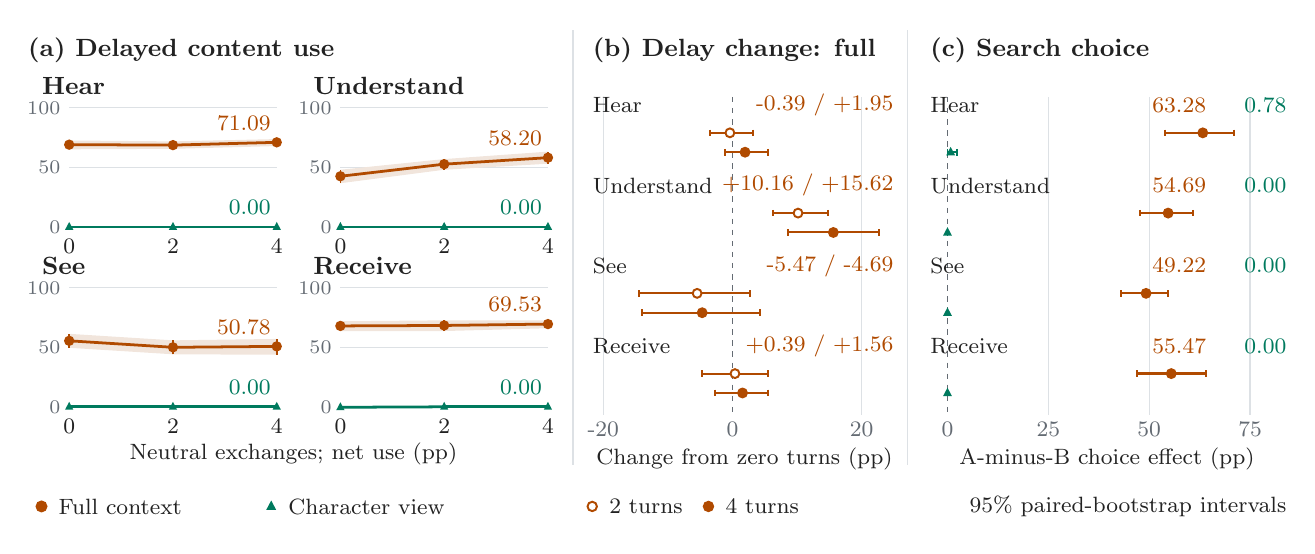
\begin{tikzpicture}[x=1pt,y=-1pt]
\path[use as bounding box] (0,0) rectangle (455,180);
\node[anchor=west,inner sep=0pt,text={rgb,255:red,34;green,34;blue,34},font=\fontsize{9}{10}\selectfont\bfseries] at (0.0000,8.0000) {(a) Delayed content use};
\node[anchor=west,inner sep=0pt,text={rgb,255:red,34;green,34;blue,34},font=\fontsize{9}{10}\selectfont\bfseries] at (204.0000,8.0000) {(b) Delay change: full};
\node[anchor=west,inner sep=0pt,text={rgb,255:red,34;green,34;blue,34},font=\fontsize{9}{10}\selectfont\bfseries] at (326.0000,8.0000) {(c) Search choice};
\draw[draw={rgb,255:red,221;green,225;blue,229},line width=0.5pt] (197.0000,1.0000)--(197.0000,158.0000);
\draw[draw={rgb,255:red,221;green,225;blue,229},line width=0.5pt] (318.0000,1.0000)--(318.0000,158.0000);
\node[anchor=west,inner sep=0pt,text={rgb,255:red,34;green,34;blue,34},font=\fontsize{8.7}{9.7}\selectfont\bfseries] at (5.0000,21.0000) {Hear};
\draw[draw={rgb,255:red,221;green,225;blue,229},line width=0.4pt] (15.0000,72.0000)--(90.0000,72.0000);
\node[anchor=east,inner sep=0pt,text={rgb,255:red,100;green,107;blue,115},font=\fontsize{7.5}{8.5}\selectfont] at (12.0000,72.0000) {0};
\draw[draw={rgb,255:red,221;green,225;blue,229},line width=0.4pt] (15.0000,50.5000)--(90.0000,50.5000);
\node[anchor=east,inner sep=0pt,text={rgb,255:red,100;green,107;blue,115},font=\fontsize{7.5}{8.5}\selectfont] at (12.0000,50.5000) {50};
\draw[draw={rgb,255:red,221;green,225;blue,229},line width=0.4pt] (15.0000,29.0000)--(90.0000,29.0000);
\node[anchor=east,inner sep=0pt,text={rgb,255:red,100;green,107;blue,115},font=\fontsize{7.5}{8.5}\selectfont] at (12.0000,29.0000) {100};
\node[anchor=center,inner sep=0pt,text={rgb,255:red,34;green,34;blue,34},font=\fontsize{8}{9}\selectfont] at (15.0000,79.0000) {0};
\node[anchor=center,inner sep=0pt,text={rgb,255:red,34;green,34;blue,34},font=\fontsize{8}{9}\selectfont] at (52.5000,79.0000) {2};
\node[anchor=center,inner sep=0pt,text={rgb,255:red,34;green,34;blue,34},font=\fontsize{8}{9}\selectfont] at (90.0000,79.0000) {4};
\fill[fill={rgb,255:red,241;green,229;blue,220}] (15.0000,40.7578)--(52.5000,41.0938)--(90.0000,40.2539)--(90.0000,42.7734)--(52.5000,43.7812)--(15.0000,43.9492)--cycle;
\draw[draw={rgb,255:red,176;green,74;blue,0},line width=0.6pt] (15.0000,43.9492)--(15.0000,40.7578);
\draw[draw={rgb,255:red,176;green,74;blue,0},fill={rgb,255:red,176;green,74;blue,0},line width=.7pt] (15.0000,42.2695) circle[radius=1.5pt];
\draw[draw={rgb,255:red,176;green,74;blue,0},line width=0.6pt] (52.5000,43.7812)--(52.5000,41.0938);
\draw[draw={rgb,255:red,176;green,74;blue,0},line width=1pt] (15.0000,42.2695)--(52.5000,42.4375);
\draw[draw={rgb,255:red,176;green,74;blue,0},fill={rgb,255:red,176;green,74;blue,0},line width=.7pt] (52.5000,42.4375) circle[radius=1.5pt];
\draw[draw={rgb,255:red,176;green,74;blue,0},line width=0.6pt] (90.0000,42.7734)--(90.0000,40.2539);
\draw[draw={rgb,255:red,176;green,74;blue,0},line width=1pt] (52.5000,42.4375)--(90.0000,41.4297);
\draw[draw={rgb,255:red,176;green,74;blue,0},fill={rgb,255:red,176;green,74;blue,0},line width=.7pt] (90.0000,41.4297) circle[radius=1.5pt];
\node[anchor=east,inner sep=0pt,text={rgb,255:red,176;green,74;blue,0},font=\fontsize{7.8}{8.8}\selectfont] at (88.0000,34.4297) {71.09};
\fill[fill={rgb,255:red,220;green,235;blue,231}] (15.0000,72.0000)--(52.5000,72.0000)--(90.0000,72.0000)--(90.0000,72.0000)--(52.5000,72.0000)--(15.0000,72.0000)--cycle;
\draw[draw={rgb,255:red,0;green,122;blue,94},line width=0.6pt] (15.0000,72.0000)--(15.0000,72.0000);
\fill[fill={rgb,255:red,0;green,122;blue,94}] (15.0000,70.2000)--(13.5000,73.0500)--(16.5000,73.0500)--cycle;
\draw[draw={rgb,255:red,0;green,122;blue,94},line width=0.6pt] (52.5000,72.0000)--(52.5000,72.0000);
\draw[draw={rgb,255:red,0;green,122;blue,94},line width=1pt] (15.0000,72.0000)--(52.5000,72.0000);
\fill[fill={rgb,255:red,0;green,122;blue,94}] (52.5000,70.2000)--(51.0000,73.0500)--(54.0000,73.0500)--cycle;
\draw[draw={rgb,255:red,0;green,122;blue,94},line width=0.6pt] (90.0000,72.0000)--(90.0000,72.0000);
\draw[draw={rgb,255:red,0;green,122;blue,94},line width=1pt] (52.5000,72.0000)--(90.0000,72.0000);
\fill[fill={rgb,255:red,0;green,122;blue,94}] (90.0000,70.2000)--(88.5000,73.0500)--(91.5000,73.0500)--cycle;
\node[anchor=east,inner sep=0pt,text={rgb,255:red,0;green,122;blue,94},font=\fontsize{7.8}{8.8}\selectfont] at (88.0000,65.0000) {0.00};
\node[anchor=west,inner sep=0pt,text={rgb,255:red,34;green,34;blue,34},font=\fontsize{8.7}{9.7}\selectfont\bfseries] at (103.0000,21.0000) {Understand};
\draw[draw={rgb,255:red,221;green,225;blue,229},line width=0.4pt] (113.0000,72.0000)--(188.0000,72.0000);
\node[anchor=east,inner sep=0pt,text={rgb,255:red,100;green,107;blue,115},font=\fontsize{7.5}{8.5}\selectfont] at (110.0000,72.0000) {0};
\draw[draw={rgb,255:red,221;green,225;blue,229},line width=0.4pt] (113.0000,50.5000)--(188.0000,50.5000);
\node[anchor=east,inner sep=0pt,text={rgb,255:red,100;green,107;blue,115},font=\fontsize{7.5}{8.5}\selectfont] at (110.0000,50.5000) {50};
\draw[draw={rgb,255:red,221;green,225;blue,229},line width=0.4pt] (113.0000,29.0000)--(188.0000,29.0000);
\node[anchor=east,inner sep=0pt,text={rgb,255:red,100;green,107;blue,115},font=\fontsize{7.5}{8.5}\selectfont] at (110.0000,29.0000) {100};
\node[anchor=center,inner sep=0pt,text={rgb,255:red,34;green,34;blue,34},font=\fontsize{8}{9}\selectfont] at (113.0000,79.0000) {0};
\node[anchor=center,inner sep=0pt,text={rgb,255:red,34;green,34;blue,34},font=\fontsize{8}{9}\selectfont] at (150.5000,79.0000) {2};
\node[anchor=center,inner sep=0pt,text={rgb,255:red,34;green,34;blue,34},font=\fontsize{8}{9}\selectfont] at (188.0000,79.0000) {4};
\fill[fill={rgb,255:red,241;green,229;blue,220}] (113.0000,51.3398)--(150.5000,47.4766)--(188.0000,44.7891)--(188.0000,49.1604)--(150.5000,51.3398)--(113.0000,56.2109)--cycle;
\draw[draw={rgb,255:red,176;green,74;blue,0},line width=0.6pt] (113.0000,56.2109)--(113.0000,51.3398);
\draw[draw={rgb,255:red,176;green,74;blue,0},fill={rgb,255:red,176;green,74;blue,0},line width=.7pt] (113.0000,53.6914) circle[radius=1.5pt];
\draw[draw={rgb,255:red,176;green,74;blue,0},line width=0.6pt] (150.5000,51.3398)--(150.5000,47.4766);
\draw[draw={rgb,255:red,176;green,74;blue,0},line width=1pt] (113.0000,53.6914)--(150.5000,49.3242);
\draw[draw={rgb,255:red,176;green,74;blue,0},fill={rgb,255:red,176;green,74;blue,0},line width=.7pt] (150.5000,49.3242) circle[radius=1.5pt];
\draw[draw={rgb,255:red,176;green,74;blue,0},line width=0.6pt] (188.0000,49.1604)--(188.0000,44.7891);
\draw[draw={rgb,255:red,176;green,74;blue,0},line width=1pt] (150.5000,49.3242)--(188.0000,46.9727);
\draw[draw={rgb,255:red,176;green,74;blue,0},fill={rgb,255:red,176;green,74;blue,0},line width=.7pt] (188.0000,46.9727) circle[radius=1.5pt];
\node[anchor=east,inner sep=0pt,text={rgb,255:red,176;green,74;blue,0},font=\fontsize{7.8}{8.8}\selectfont] at (186.0000,39.9727) {58.20};
\fill[fill={rgb,255:red,220;green,235;blue,231}] (113.0000,72.0000)--(150.5000,72.0000)--(188.0000,72.0000)--(188.0000,72.0000)--(150.5000,72.0000)--(113.0000,72.0000)--cycle;
\draw[draw={rgb,255:red,0;green,122;blue,94},line width=0.6pt] (113.0000,72.0000)--(113.0000,72.0000);
\fill[fill={rgb,255:red,0;green,122;blue,94}] (113.0000,70.2000)--(111.5000,73.0500)--(114.5000,73.0500)--cycle;
\draw[draw={rgb,255:red,0;green,122;blue,94},line width=0.6pt] (150.5000,72.0000)--(150.5000,72.0000);
\draw[draw={rgb,255:red,0;green,122;blue,94},line width=1pt] (113.0000,72.0000)--(150.5000,72.0000);
\fill[fill={rgb,255:red,0;green,122;blue,94}] (150.5000,70.2000)--(149.0000,73.0500)--(152.0000,73.0500)--cycle;
\draw[draw={rgb,255:red,0;green,122;blue,94},line width=0.6pt] (188.0000,72.0000)--(188.0000,72.0000);
\draw[draw={rgb,255:red,0;green,122;blue,94},line width=1pt] (150.5000,72.0000)--(188.0000,72.0000);
\fill[fill={rgb,255:red,0;green,122;blue,94}] (188.0000,70.2000)--(186.5000,73.0500)--(189.5000,73.0500)--cycle;
\node[anchor=east,inner sep=0pt,text={rgb,255:red,0;green,122;blue,94},font=\fontsize{7.8}{8.8}\selectfont] at (186.0000,65.0000) {0.00};
\node[anchor=west,inner sep=0pt,text={rgb,255:red,34;green,34;blue,34},font=\fontsize{8.7}{9.7}\selectfont\bfseries] at (5.0000,86.0000) {See};
\draw[draw={rgb,255:red,221;green,225;blue,229},line width=0.4pt] (15.0000,137.0000)--(90.0000,137.0000);
\node[anchor=east,inner sep=0pt,text={rgb,255:red,100;green,107;blue,115},font=\fontsize{7.5}{8.5}\selectfont] at (12.0000,137.0000) {0};
\draw[draw={rgb,255:red,221;green,225;blue,229},line width=0.4pt] (15.0000,115.5000)--(90.0000,115.5000);
\node[anchor=east,inner sep=0pt,text={rgb,255:red,100;green,107;blue,115},font=\fontsize{7.5}{8.5}\selectfont] at (12.0000,115.5000) {50};
\draw[draw={rgb,255:red,221;green,225;blue,229},line width=0.4pt] (15.0000,94.0000)--(90.0000,94.0000);
\node[anchor=east,inner sep=0pt,text={rgb,255:red,100;green,107;blue,115},font=\fontsize{7.5}{8.5}\selectfont] at (12.0000,94.0000) {100};
\node[anchor=center,inner sep=0pt,text={rgb,255:red,34;green,34;blue,34},font=\fontsize{8}{9}\selectfont] at (15.0000,144.0000) {0};
\node[anchor=center,inner sep=0pt,text={rgb,255:red,34;green,34;blue,34},font=\fontsize{8}{9}\selectfont] at (52.5000,144.0000) {2};
\node[anchor=center,inner sep=0pt,text={rgb,255:red,34;green,34;blue,34},font=\fontsize{8}{9}\selectfont] at (90.0000,144.0000) {4};
\fill[fill={rgb,255:red,241;green,229;blue,220}] (15.0000,110.6289)--(52.5000,112.9805)--(90.0000,112.4766)--(90.0000,118.1875)--(52.5000,118.0195)--(15.0000,115.6680)--cycle;
\draw[draw={rgb,255:red,176;green,74;blue,0},line width=0.6pt] (15.0000,115.6680)--(15.0000,110.6289);
\draw[draw={rgb,255:red,176;green,74;blue,0},fill={rgb,255:red,176;green,74;blue,0},line width=.7pt] (15.0000,113.1484) circle[radius=1.5pt];
\draw[draw={rgb,255:red,176;green,74;blue,0},line width=0.6pt] (52.5000,118.0195)--(52.5000,112.9805);
\draw[draw={rgb,255:red,176;green,74;blue,0},line width=1pt] (15.0000,113.1484)--(52.5000,115.5000);
\draw[draw={rgb,255:red,176;green,74;blue,0},fill={rgb,255:red,176;green,74;blue,0},line width=.7pt] (52.5000,115.5000) circle[radius=1.5pt];
\draw[draw={rgb,255:red,176;green,74;blue,0},line width=0.6pt] (90.0000,118.1875)--(90.0000,112.4766);
\draw[draw={rgb,255:red,176;green,74;blue,0},line width=1pt] (52.5000,115.5000)--(90.0000,115.1641);
\draw[draw={rgb,255:red,176;green,74;blue,0},fill={rgb,255:red,176;green,74;blue,0},line width=.7pt] (90.0000,115.1641) circle[radius=1.5pt];
\node[anchor=east,inner sep=0pt,text={rgb,255:red,176;green,74;blue,0},font=\fontsize{7.8}{8.8}\selectfont] at (88.0000,108.1641) {50.78};
\fill[fill={rgb,255:red,220;green,235;blue,231}] (15.0000,137.0000)--(52.5000,137.0000)--(90.0000,137.0000)--(90.0000,137.0000)--(52.5000,137.0000)--(15.0000,137.0000)--cycle;
\draw[draw={rgb,255:red,0;green,122;blue,94},line width=0.6pt] (15.0000,137.0000)--(15.0000,137.0000);
\fill[fill={rgb,255:red,0;green,122;blue,94}] (15.0000,135.2000)--(13.5000,138.0500)--(16.5000,138.0500)--cycle;
\draw[draw={rgb,255:red,0;green,122;blue,94},line width=0.6pt] (52.5000,137.0000)--(52.5000,137.0000);
\draw[draw={rgb,255:red,0;green,122;blue,94},line width=1pt] (15.0000,137.0000)--(52.5000,137.0000);
\fill[fill={rgb,255:red,0;green,122;blue,94}] (52.5000,135.2000)--(51.0000,138.0500)--(54.0000,138.0500)--cycle;
\draw[draw={rgb,255:red,0;green,122;blue,94},line width=0.6pt] (90.0000,137.0000)--(90.0000,137.0000);
\draw[draw={rgb,255:red,0;green,122;blue,94},line width=1pt] (52.5000,137.0000)--(90.0000,137.0000);
\fill[fill={rgb,255:red,0;green,122;blue,94}] (90.0000,135.2000)--(88.5000,138.0500)--(91.5000,138.0500)--cycle;
\node[anchor=east,inner sep=0pt,text={rgb,255:red,0;green,122;blue,94},font=\fontsize{7.8}{8.8}\selectfont] at (88.0000,130.0000) {0.00};
\node[anchor=west,inner sep=0pt,text={rgb,255:red,34;green,34;blue,34},font=\fontsize{8.7}{9.7}\selectfont\bfseries] at (103.0000,86.0000) {Receive};
\draw[draw={rgb,255:red,221;green,225;blue,229},line width=0.4pt] (113.0000,137.0000)--(188.0000,137.0000);
\node[anchor=east,inner sep=0pt,text={rgb,255:red,100;green,107;blue,115},font=\fontsize{7.5}{8.5}\selectfont] at (110.0000,137.0000) {0};
\draw[draw={rgb,255:red,221;green,225;blue,229},line width=0.4pt] (113.0000,115.5000)--(188.0000,115.5000);
\node[anchor=east,inner sep=0pt,text={rgb,255:red,100;green,107;blue,115},font=\fontsize{7.5}{8.5}\selectfont] at (110.0000,115.5000) {50};
\draw[draw={rgb,255:red,221;green,225;blue,229},line width=0.4pt] (113.0000,94.0000)--(188.0000,94.0000);
\node[anchor=east,inner sep=0pt,text={rgb,255:red,100;green,107;blue,115},font=\fontsize{7.5}{8.5}\selectfont] at (110.0000,94.0000) {100};
\node[anchor=center,inner sep=0pt,text={rgb,255:red,34;green,34;blue,34},font=\fontsize{8}{9}\selectfont] at (113.0000,144.0000) {0};
\node[anchor=center,inner sep=0pt,text={rgb,255:red,34;green,34;blue,34},font=\fontsize{8}{9}\selectfont] at (150.5000,144.0000) {2};
\node[anchor=center,inner sep=0pt,text={rgb,255:red,34;green,34;blue,34},font=\fontsize{8}{9}\selectfont] at (188.0000,144.0000) {4};
\fill[fill={rgb,255:red,241;green,229;blue,220}] (113.0000,106.0896)--(150.5000,105.7578)--(188.0000,105.7578)--(188.0000,108.6133)--(150.5000,109.6211)--(113.0000,109.6211)--cycle;
\draw[draw={rgb,255:red,176;green,74;blue,0},line width=0.6pt] (113.0000,109.6211)--(113.0000,106.0896);
\draw[draw={rgb,255:red,176;green,74;blue,0},fill={rgb,255:red,176;green,74;blue,0},line width=.7pt] (113.0000,107.7734) circle[radius=1.5pt];
\draw[draw={rgb,255:red,176;green,74;blue,0},line width=0.6pt] (150.5000,109.6211)--(150.5000,105.7578);
\draw[draw={rgb,255:red,176;green,74;blue,0},line width=1pt] (113.0000,107.7734)--(150.5000,107.6055);
\draw[draw={rgb,255:red,176;green,74;blue,0},fill={rgb,255:red,176;green,74;blue,0},line width=.7pt] (150.5000,107.6055) circle[radius=1.5pt];
\draw[draw={rgb,255:red,176;green,74;blue,0},line width=0.6pt] (188.0000,108.6133)--(188.0000,105.7578);
\draw[draw={rgb,255:red,176;green,74;blue,0},line width=1pt] (150.5000,107.6055)--(188.0000,107.1016);
\draw[draw={rgb,255:red,176;green,74;blue,0},fill={rgb,255:red,176;green,74;blue,0},line width=.7pt] (188.0000,107.1016) circle[radius=1.5pt];
\node[anchor=east,inner sep=0pt,text={rgb,255:red,176;green,74;blue,0},font=\fontsize{7.8}{8.8}\selectfont] at (186.0000,100.1016) {69.53};
\fill[fill={rgb,255:red,220;green,235;blue,231}] (113.0000,137.0000)--(150.5000,137.0000)--(188.0000,137.0000)--(188.0000,137.0000)--(150.5000,137.0000)--(113.0000,137.5039)--cycle;
\draw[draw={rgb,255:red,0;green,122;blue,94},line width=0.6pt] (113.0000,137.5039)--(113.0000,137.0000);
\fill[fill={rgb,255:red,0;green,122;blue,94}] (113.0000,135.3680)--(111.5000,138.2180)--(114.5000,138.2180)--cycle;
\draw[draw={rgb,255:red,0;green,122;blue,94},line width=0.6pt] (150.5000,137.0000)--(150.5000,137.0000);
\draw[draw={rgb,255:red,0;green,122;blue,94},line width=1pt] (113.0000,137.1680)--(150.5000,137.0000);
\fill[fill={rgb,255:red,0;green,122;blue,94}] (150.5000,135.2000)--(149.0000,138.0500)--(152.0000,138.0500)--cycle;
\draw[draw={rgb,255:red,0;green,122;blue,94},line width=0.6pt] (188.0000,137.0000)--(188.0000,137.0000);
\draw[draw={rgb,255:red,0;green,122;blue,94},line width=1pt] (150.5000,137.0000)--(188.0000,137.0000);
\fill[fill={rgb,255:red,0;green,122;blue,94}] (188.0000,135.2000)--(186.5000,138.0500)--(189.5000,138.0500)--cycle;
\node[anchor=east,inner sep=0pt,text={rgb,255:red,0;green,122;blue,94},font=\fontsize{7.8}{8.8}\selectfont] at (186.0000,130.0000) {0.00};
\node[anchor=center,inner sep=0pt,text={rgb,255:red,34;green,34;blue,34},font=\fontsize{8.5}{9.5}\selectfont] at (96.0000,154.0000) {Neutral exchanges; net use (pp)};
\draw[draw={rgb,255:red,221;green,225;blue,229},line width=0.5pt] (208.0000,25.0000)--(208.0000,140.0000);
\node[anchor=center,inner sep=0pt,text={rgb,255:red,100;green,107;blue,115},font=\fontsize{8}{9}\selectfont] at (208.0000,145.0000) {-20};
\draw[draw={rgb,255:red,100;green,107;blue,115},line width=0.5pt,dash pattern=on 2pt off 2pt] (254.6667,25.0000)--(254.6667,140.0000);
\node[anchor=center,inner sep=0pt,text={rgb,255:red,100;green,107;blue,115},font=\fontsize{8}{9}\selectfont] at (254.6667,145.0000) {0};
\draw[draw={rgb,255:red,221;green,225;blue,229},line width=0.5pt] (301.3333,25.0000)--(301.3333,140.0000);
\node[anchor=center,inner sep=0pt,text={rgb,255:red,100;green,107;blue,115},font=\fontsize{8}{9}\selectfont] at (301.3333,145.0000) {20};
\draw[draw={rgb,255:red,176;green,74;blue,0},line width=0.7pt] (246.4635,38.0000)--(261.9583,38.0000);
\draw[draw={rgb,255:red,176;green,74;blue,0},line width=0.65pt] (246.4635,36.8000)--(246.4635,39.2000);
\draw[draw={rgb,255:red,176;green,74;blue,0},line width=0.65pt] (261.9583,36.8000)--(261.9583,39.2000);
\draw[draw={rgb,255:red,176;green,74;blue,0},fill={rgb,255:red,255;green,255;blue,255},line width=.7pt] (253.7552,38.0000) circle[radius=1.6pt];
\draw[draw={rgb,255:red,176;green,74;blue,0},line width=0.7pt] (251.9323,45.0000)--(267.4271,45.0000);
\draw[draw={rgb,255:red,176;green,74;blue,0},line width=0.65pt] (251.9323,43.8000)--(251.9323,46.2000);
\draw[draw={rgb,255:red,176;green,74;blue,0},line width=0.65pt] (267.4271,43.8000)--(267.4271,46.2000);
\draw[draw={rgb,255:red,176;green,74;blue,0},fill={rgb,255:red,176;green,74;blue,0},line width=.7pt] (259.2240,45.0000) circle[radius=1.6pt];
\node[anchor=west,inner sep=0pt,text={rgb,255:red,34;green,34;blue,34},font=\fontsize{8.3}{9.3}\selectfont] at (204.0000,28.0000) {Hear};
\node[anchor=east,inner sep=0pt,text={rgb,255:red,176;green,74;blue,0},font=\fontsize{8}{9}\selectfont] at (313.0000,28.0000) {-0.39 / +1.95};
\draw[draw={rgb,255:red,176;green,74;blue,0},line width=0.7pt] (269.2500,67.0000)--(289.3021,67.0000);
\draw[draw={rgb,255:red,176;green,74;blue,0},line width=0.65pt] (269.2500,65.8000)--(269.2500,68.2000);
\draw[draw={rgb,255:red,176;green,74;blue,0},line width=0.65pt] (289.3021,65.8000)--(289.3021,68.2000);
\draw[draw={rgb,255:red,176;green,74;blue,0},fill={rgb,255:red,255;green,255;blue,255},line width=.7pt] (278.3646,67.0000) circle[radius=1.6pt];
\draw[draw={rgb,255:red,176;green,74;blue,0},line width=0.7pt] (274.7188,74.0000)--(307.5312,74.0000);
\draw[draw={rgb,255:red,176;green,74;blue,0},line width=0.65pt] (274.7188,72.8000)--(274.7188,75.2000);
\draw[draw={rgb,255:red,176;green,74;blue,0},line width=0.65pt] (307.5312,72.8000)--(307.5312,75.2000);
\draw[draw={rgb,255:red,176;green,74;blue,0},fill={rgb,255:red,176;green,74;blue,0},line width=.7pt] (291.1250,74.0000) circle[radius=1.6pt];
\node[anchor=west,inner sep=0pt,text={rgb,255:red,34;green,34;blue,34},font=\fontsize{8.3}{9.3}\selectfont] at (204.0000,57.0000) {Understand};
\node[anchor=east,inner sep=0pt,text={rgb,255:red,176;green,74;blue,0},font=\fontsize{8}{9}\selectfont] at (313.0000,57.0000) {+10.16 / +15.62};
\draw[draw={rgb,255:red,176;green,74;blue,0},line width=0.7pt] (220.9427,96.0000)--(261.0469,96.0000);
\draw[draw={rgb,255:red,176;green,74;blue,0},line width=0.65pt] (220.9427,94.8000)--(220.9427,97.2000);
\draw[draw={rgb,255:red,176;green,74;blue,0},line width=0.65pt] (261.0469,94.8000)--(261.0469,97.2000);
\draw[draw={rgb,255:red,176;green,74;blue,0},fill={rgb,255:red,255;green,255;blue,255},line width=.7pt] (241.9062,96.0000) circle[radius=1.6pt];
\draw[draw={rgb,255:red,176;green,74;blue,0},line width=0.7pt] (221.8542,103.0000)--(264.6927,103.0000);
\draw[draw={rgb,255:red,176;green,74;blue,0},line width=0.65pt] (221.8542,101.8000)--(221.8542,104.2000);
\draw[draw={rgb,255:red,176;green,74;blue,0},line width=0.65pt] (264.6927,101.8000)--(264.6927,104.2000);
\draw[draw={rgb,255:red,176;green,74;blue,0},fill={rgb,255:red,176;green,74;blue,0},line width=.7pt] (243.7292,103.0000) circle[radius=1.6pt];
\node[anchor=west,inner sep=0pt,text={rgb,255:red,34;green,34;blue,34},font=\fontsize{8.3}{9.3}\selectfont] at (204.0000,86.0000) {See};
\node[anchor=east,inner sep=0pt,text={rgb,255:red,176;green,74;blue,0},font=\fontsize{8}{9}\selectfont] at (313.0000,86.0000) {-5.47 / -4.69};
\draw[draw={rgb,255:red,176;green,74;blue,0},line width=0.7pt] (243.7292,125.0000)--(267.4271,125.0000);
\draw[draw={rgb,255:red,176;green,74;blue,0},line width=0.65pt] (243.7292,123.8000)--(243.7292,126.2000);
\draw[draw={rgb,255:red,176;green,74;blue,0},line width=0.65pt] (267.4271,123.8000)--(267.4271,126.2000);
\draw[draw={rgb,255:red,176;green,74;blue,0},fill={rgb,255:red,255;green,255;blue,255},line width=.7pt] (255.5781,125.0000) circle[radius=1.6pt];
\draw[draw={rgb,255:red,176;green,74;blue,0},line width=0.7pt] (248.2865,132.0000)--(267.4271,132.0000);
\draw[draw={rgb,255:red,176;green,74;blue,0},line width=0.65pt] (248.2865,130.8000)--(248.2865,133.2000);
\draw[draw={rgb,255:red,176;green,74;blue,0},line width=0.65pt] (267.4271,130.8000)--(267.4271,133.2000);
\draw[draw={rgb,255:red,176;green,74;blue,0},fill={rgb,255:red,176;green,74;blue,0},line width=.7pt] (258.3125,132.0000) circle[radius=1.6pt];
\node[anchor=west,inner sep=0pt,text={rgb,255:red,34;green,34;blue,34},font=\fontsize{8.3}{9.3}\selectfont] at (204.0000,115.0000) {Receive};
\node[anchor=east,inner sep=0pt,text={rgb,255:red,176;green,74;blue,0},font=\fontsize{8}{9}\selectfont] at (313.0000,115.0000) {+0.39 / +1.56};
\node[anchor=center,inner sep=0pt,text={rgb,255:red,34;green,34;blue,34},font=\fontsize{8.2}{9.2}\selectfont] at (259.0000,156.0000) {Change from zero turns (pp)};
\draw[draw={rgb,255:red,100;green,107;blue,115},line width=0.5pt,dash pattern=on 2pt off 2pt] (332.3735,25.0000)--(332.3735,140.0000);
\node[anchor=center,inner sep=0pt,text={rgb,255:red,100;green,107;blue,115},font=\fontsize{8}{9}\selectfont] at (332.3735,145.0000) {0};
\draw[draw={rgb,255:red,221;green,225;blue,229},line width=0.5pt] (368.8193,25.0000)--(368.8193,140.0000);
\node[anchor=center,inner sep=0pt,text={rgb,255:red,100;green,107;blue,115},font=\fontsize{8}{9}\selectfont] at (368.8193,145.0000) {25};
\draw[draw={rgb,255:red,221;green,225;blue,229},line width=0.5pt] (405.2651,25.0000)--(405.2651,140.0000);
\node[anchor=center,inner sep=0pt,text={rgb,255:red,100;green,107;blue,115},font=\fontsize{8}{9}\selectfont] at (405.2651,145.0000) {50};
\draw[draw={rgb,255:red,221;green,225;blue,229},line width=0.5pt] (441.7108,25.0000)--(441.7108,140.0000);
\node[anchor=center,inner sep=0pt,text={rgb,255:red,100;green,107;blue,115},font=\fontsize{8}{9}\selectfont] at (441.7108,145.0000) {75};
\node[anchor=west,inner sep=0pt,text={rgb,255:red,34;green,34;blue,34},font=\fontsize{8.3}{9.3}\selectfont] at (326.0000,28.0000) {Hear};
\draw[draw={rgb,255:red,176;green,74;blue,0},line width=0.8pt] (410.9597,38.0000)--(436.0162,38.0000);
\draw[draw={rgb,255:red,176;green,74;blue,0},line width=0.65pt] (410.9597,36.8000)--(410.9597,39.2000);
\draw[draw={rgb,255:red,176;green,74;blue,0},line width=0.65pt] (436.0162,36.8000)--(436.0162,39.2000);
\draw[draw={rgb,255:red,176;green,74;blue,0},fill={rgb,255:red,176;green,74;blue,0},line width=.7pt] (424.6269,38.0000) circle[radius=1.6pt];
\node[anchor=east,inner sep=0pt,text={rgb,255:red,176;green,74;blue,0},font=\fontsize{8}{9}\selectfont] at (426.0000,28.0000) {63.28};
\draw[draw={rgb,255:red,0;green,122;blue,94},line width=0.8pt] (332.3735,45.0000)--(335.7903,45.0000);
\draw[draw={rgb,255:red,0;green,122;blue,94},line width=0.65pt] (332.3735,43.8000)--(332.3735,46.2000);
\draw[draw={rgb,255:red,0;green,122;blue,94},line width=0.65pt] (335.7903,43.8000)--(335.7903,46.2000);
\fill[fill={rgb,255:red,0;green,122;blue,94}] (333.5124,43.0800)--(331.9124,46.1200)--(335.1124,46.1200)--cycle;
\node[anchor=east,inner sep=0pt,text={rgb,255:red,0;green,122;blue,94},font=\fontsize{8}{9}\selectfont] at (455.0000,28.0000) {0.78};
\node[anchor=west,inner sep=0pt,text={rgb,255:red,34;green,34;blue,34},font=\fontsize{8.3}{9.3}\selectfont] at (326.0000,57.0000) {Understand};
\draw[draw={rgb,255:red,176;green,74;blue,0},line width=0.8pt] (401.8483,67.0000)--(421.2101,67.0000);
\draw[draw={rgb,255:red,176;green,74;blue,0},line width=0.65pt] (401.8483,65.8000)--(401.8483,68.2000);
\draw[draw={rgb,255:red,176;green,74;blue,0},line width=0.65pt] (421.2101,65.8000)--(421.2101,68.2000);
\draw[draw={rgb,255:red,176;green,74;blue,0},fill={rgb,255:red,176;green,74;blue,0},line width=.7pt] (412.0986,67.0000) circle[radius=1.6pt];
\node[anchor=east,inner sep=0pt,text={rgb,255:red,176;green,74;blue,0},font=\fontsize{8}{9}\selectfont] at (426.0000,57.0000) {54.69};
\draw[draw={rgb,255:red,0;green,122;blue,94},line width=0.8pt] (332.3735,74.0000)--(332.3735,74.0000);
\draw[draw={rgb,255:red,0;green,122;blue,94},line width=0.65pt] (332.3735,72.8000)--(332.3735,75.2000);
\draw[draw={rgb,255:red,0;green,122;blue,94},line width=0.65pt] (332.3735,72.8000)--(332.3735,75.2000);
\fill[fill={rgb,255:red,0;green,122;blue,94}] (332.3735,72.0800)--(330.7735,75.1200)--(333.9735,75.1200)--cycle;
\node[anchor=east,inner sep=0pt,text={rgb,255:red,0;green,122;blue,94},font=\fontsize{8}{9}\selectfont] at (455.0000,57.0000) {0.00};
\node[anchor=west,inner sep=0pt,text={rgb,255:red,34;green,34;blue,34},font=\fontsize{8.3}{9.3}\selectfont] at (326.0000,86.0000) {See};
\draw[draw={rgb,255:red,176;green,74;blue,0},line width=0.8pt] (395.0147,96.0000)--(412.0986,96.0000);
\draw[draw={rgb,255:red,176;green,74;blue,0},line width=0.65pt] (395.0147,94.8000)--(395.0147,97.2000);
\draw[draw={rgb,255:red,176;green,74;blue,0},line width=0.65pt] (412.0986,94.8000)--(412.0986,97.2000);
\draw[draw={rgb,255:red,176;green,74;blue,0},fill={rgb,255:red,176;green,74;blue,0},line width=.7pt] (404.1261,96.0000) circle[radius=1.6pt];
\node[anchor=east,inner sep=0pt,text={rgb,255:red,176;green,74;blue,0},font=\fontsize{8}{9}\selectfont] at (426.0000,86.0000) {49.22};
\draw[draw={rgb,255:red,0;green,122;blue,94},line width=0.8pt] (332.3735,103.0000)--(332.3735,103.0000);
\draw[draw={rgb,255:red,0;green,122;blue,94},line width=0.65pt] (332.3735,101.8000)--(332.3735,104.2000);
\draw[draw={rgb,255:red,0;green,122;blue,94},line width=0.65pt] (332.3735,101.8000)--(332.3735,104.2000);
\fill[fill={rgb,255:red,0;green,122;blue,94}] (332.3735,101.0800)--(330.7735,104.1200)--(333.9735,104.1200)--cycle;
\node[anchor=east,inner sep=0pt,text={rgb,255:red,0;green,122;blue,94},font=\fontsize{8}{9}\selectfont] at (455.0000,86.0000) {0.00};
\node[anchor=west,inner sep=0pt,text={rgb,255:red,34;green,34;blue,34},font=\fontsize{8.3}{9.3}\selectfont] at (326.0000,115.0000) {Receive};
\draw[draw={rgb,255:red,176;green,74;blue,0},line width=0.8pt] (400.7093,125.0000)--(425.7658,125.0000);
\draw[draw={rgb,255:red,176;green,74;blue,0},line width=0.65pt] (400.7093,123.8000)--(400.7093,126.2000);
\draw[draw={rgb,255:red,176;green,74;blue,0},line width=0.65pt] (425.7658,123.8000)--(425.7658,126.2000);
\draw[draw={rgb,255:red,176;green,74;blue,0},fill={rgb,255:red,176;green,74;blue,0},line width=.7pt] (413.2376,125.0000) circle[radius=1.6pt];
\node[anchor=east,inner sep=0pt,text={rgb,255:red,176;green,74;blue,0},font=\fontsize{8}{9}\selectfont] at (426.0000,115.0000) {55.47};
\draw[draw={rgb,255:red,0;green,122;blue,94},line width=0.8pt] (332.3735,132.0000)--(332.3735,132.0000);
\draw[draw={rgb,255:red,0;green,122;blue,94},line width=0.65pt] (332.3735,130.8000)--(332.3735,133.2000);
\draw[draw={rgb,255:red,0;green,122;blue,94},line width=0.65pt] (332.3735,130.8000)--(332.3735,133.2000);
\fill[fill={rgb,255:red,0;green,122;blue,94}] (332.3735,130.0800)--(330.7735,133.1200)--(333.9735,133.1200)--cycle;
\node[anchor=east,inner sep=0pt,text={rgb,255:red,0;green,122;blue,94},font=\fontsize{8}{9}\selectfont] at (455.0000,115.0000) {0.00};
\node[anchor=center,inner sep=0pt,text={rgb,255:red,34;green,34;blue,34},font=\fontsize{8.2}{9.2}\selectfont] at (390.0000,156.0000) {A-minus-B choice effect (pp)};
\draw[draw={rgb,255:red,176;green,74;blue,0},fill={rgb,255:red,176;green,74;blue,0},line width=.7pt] (5.0000,173.0000) circle[radius=1.8pt];
\node[anchor=west,inner sep=0pt,text={rgb,255:red,34;green,34;blue,34},font=\fontsize{8.5}{9.5}\selectfont] at (11.0000,173.0000) {Full context};
\fill[fill={rgb,255:red,0;green,122;blue,94}] (88.0000,170.8400)--(86.2000,174.2600)--(89.8000,174.2600)--cycle;
\node[anchor=west,inner sep=0pt,text={rgb,255:red,34;green,34;blue,34},font=\fontsize{8.5}{9.5}\selectfont] at (94.0000,173.0000) {Character view};
\draw[draw={rgb,255:red,176;green,74;blue,0},fill={rgb,255:red,255;green,255;blue,255},line width=.7pt] (204.0000,173.0000) circle[radius=1.7pt];
\node[anchor=west,inner sep=0pt,text={rgb,255:red,34;green,34;blue,34},font=\fontsize{8}{9}\selectfont] at (210.0000,173.0000) {2 turns};
\draw[draw={rgb,255:red,176;green,74;blue,0},fill={rgb,255:red,176;green,74;blue,0},line width=.7pt] (246.0000,173.0000) circle[radius=1.7pt];
\node[anchor=west,inner sep=0pt,text={rgb,255:red,34;green,34;blue,34},font=\fontsize{8}{9}\selectfont] at (252.0000,173.0000) {4 turns};
\node[anchor=east,inner sep=0pt,text={rgb,255:red,34;green,34;blue,34},font=\fontsize{8}{9}\selectfont] at (455.0000,173.0000) {95\% paired-bootstrap intervals};
\end{tikzpicture}
\end{lrbox}
\ifdim\wd\OCfigure>\linewidth\PackageError{access-paper}{Figure fig:behavior exceeds its column}{Revise the figure layout.}\fi
\usebox{\OCfigure}
\caption{Study 2, four confirmation models, 32 scenes. (a) Net use after zero, two or four neutral exchanges; (b) change from zero exchanges under full context; (c) change in choosing location A when the inaccessible fact switches from B to A. Bars are 95\% skeleton-bootstrap intervals.}
\label{fig:behavior}
\end{figure*}

\paragraph{Leaked facts persist and change choices.} With the event still in context, leakage remains 51--71 pp after four neutral exchanges; for comprehension it grows by 15.6 pp [8.6, 22.7]. When characters choose between two places to search, switching the inaccessible fact from B to A changes the choice of A by 49--63 pp under full context, against 0--1 pp under the character view, with valid answers in over 96\% of replies (Figure~\ref{fig:behavior}).

\paragraph{Methods.} In the confirmation set both removal and the character view bring leakage to 0.03 pp, and the view keeps accessible use within the locked margin ($+$0.5 pp [$-$0.2, 1.2]; Table~\ref{tab:methods}); over all 11 models the view removes 60.7 pp of leakage and changes accessible use by $+$0.6 pp [0.2, 1.0]. The view differs from removal in what the character can still report: because it keeps the observable shell, characters say they noticed the actor in all partially observable scenes, against 32\% under removal. Self-filtering, the prompted counterpart, reduces leakage but discards accessible content in some models: Qwen3.8-27B's use of content it is allowed to understand falls from 86\% to 0\% because the filter returns only ``Casey says something in Japanese'' (Appendix~\ref{app:s2}).

\begin{table}[t]
\centering\footnotesize\setlength{\tabcolsep}{3.5pt}
\begin{tabular}{@{}lrrrr@{}}
\toprule
Model & Hear & Understand & See & Receive\\
\midrule
Gemma-4-31B$^\ast$ & 5.5 & 0.0 & 16.4 & 22.4\\
Qwen3.8-27B & 22.4 & 2.6 & 41.4 & 14.8\\
Mistral-Small-24B & 95.6 & 1.6 & 31.0 & 83.3\\
Gemma-4-12B & 99.5 & 14.1 & 24.0 & 78.6\\
Seed-OSS-36B & 59.6 & 58.6 & 53.1 & 60.4\\
GLM-4.7-Flash$^\ast$ & 87.2 & 71.1 & 66.4 & 52.6\\
Falcon-H1-34B & 64.1 & 74.7 & 54.9 & 97.9\\
Phi-4 & 97.1 & 14.1 & 93.5 & 98.2\\
gpt-oss-20b & 94.8 & 37.2 & 91.4 & 88.8\\
Qwen3.5-9B$^\ast$ & 97.4 & 51.3 & 96.6 & 96.4\\
Nemotron-3-Nano$^\ast$ & 99.0 & 66.4 & 97.7 & 99.0\\
\midrule
All 11 models & 74.7 & 35.6 & 60.6 & 72.0\\
7 added models & 76.2 & 29.0 & 55.6 & 74.6\\
\bottomrule
\end{tabular}
\caption{Study 2 confirmation set (96 original-character scenes), net use of inaccessible content under full context (pp). $^\ast$Locked four-model cohort.}
\label{tab:s2ext}
\end{table}
\begin{table*}[t]
\centering\small
\begin{lrbox}{\OCtable}\begin{tabular}{@{}lrrcr@{}}
\toprule
Family / component & Estimate (pp) & 95\% CI & Null & Holm $p$\\
\midrule
C1: Hear & 72.27 & [70.90, 73.57] & 0 & 0.0015\\
C1: Understand & 47.20 & [44.86, 49.61] & 0 & ---\\
C1: See & 69.27 & [67.25, 71.35] & 0 & ---\\
C1: Receive & 67.58 & [65.82, 69.34] & 0 & ---\\
C2: State-correct net use & 63.95 & [62.73, 65.19] & 0 & 0.0015\\
\midrule
C3: Full minus view leakage & 64.05 & [62.81, 65.27] & 0 & 0.0015\\
View minus full accessible use & 0.49 & [-0.18, 1.19] & $-5$ & ---\\
View minus hard event retention & 67.75 & [65.36, 70.05] & 0 & ---\\
\bottomrule
\end{tabular}\end{lrbox}
\ifdim\wd\OCtable>\linewidth\PackageError{access-paper}{Table tab:confirm exceeds its column}{Revise the table layout.}\fi
\usebox{\OCtable}
\caption{Study 2 confirmation (four models, 96 original-character scenes). C1 requires all four channels to be positive, C2 uses replies whose state probe is correct (6,068), and C3 requires the view to reduce leakage, keep accessible use within 5 pp, and keep more observations than removal. One Holm-adjusted $p$ per family.}
\label{tab:confirm}
\end{table*}

\section{What Makes Models Comply?}
\label{sec:format}
The same two models keep the hearing boundary in Study~2 and break it in Study~1. We ran two experiments to find out why, both on the hearing channel with the boundary given as a direct flag.

\paragraph{From Study~1 toward Study~2.} Starting from Study~1's flag-only prompts, we added three features of Study~2 in a $2\times2\times2$ design: a field naming the tested channel, the direct question about the item and its location, and a minimal context without the character sheet and scene description (four models, 96 skeletons, the content question, with matched accessible controls). Naming the channel changes leakage by at most 2 pp, and the direct question by 2.7--4.0 pp. Removing the character sheet and description lowers leakage by 11.0 pp [8.0, 14.1] for unheard speech and 21.5 pp [18.1, 24.8] for speech not understood, while use of accessible speech rises slightly. Even with all three features, Gemma-4-31B still uses unheard speech in 50\% of replies.

\paragraph{From Study~2 toward Study~1.} Starting from Study~2's prompts, we swapped in one Study~1 feature at a time: its system prompt, its character sheet, its state layout (a language state and a speech event with speaker, addressee and text), or its question from a companion who missed the speech (Table~\ref{tab:bridge}). Each strong model breaks on a different swap. Gemma-4-31B goes from 0 to 62 pp when only the state layout changes, and to 100 pp with all four swaps. Qwen3.8-27B goes from 9 to 68 pp when only the character sheet changes. Phi-4 leaks under every variant. Throughout, the same models use audible speech in 80--100\% of replies, so the low leakage under Study~2's prompt reflects the boundary rather than general reticence.

\begin{table*}[t]
\centering\small
\begin{tabular}{@{}lrrrrrr@{}}
\toprule
Model & Study 2 prompt & + S1 system & + S1 sheet & + S1 state & + S1 question & All four\\
\midrule
Gemma-4-31B & 0.0 & 0.0 & 1.0 & 61.5 & 14.1 & 100.0\\
Qwen3.8-27B & 9.4 & 9.9 & 67.7 & 19.3 & 8.9 & 77.6\\
Phi-4 & 98.4 & 95.3 & 94.3 & 85.9 & 100.0 & 100.0\\
\midrule
Gemma-4-31B (heard) & 95.3 & 93.2 & 90.1 & 83.3 & 100.0 & 100.0\\
Qwen3.8-27B (heard) & 79.7 & 86.5 & 97.9 & 83.9 & 100.0 & 98.4\\
Phi-4 (heard) & 100.0 & 100.0 & 96.9 & 93.2 & 100.0 & 100.0\\
\bottomrule
\end{tabular}
\caption{Bridge experiment on Study 2's hearing prompts (96 scenes). Each column swaps in one Study 1 feature; the last swaps in all four. Top: net use of unheard speech (pp); bottom: use of the same speech when audible (\%).}
\label{tab:bridge}
\end{table*}

No single feature explains compliance. Compliance in the strongest models depends on incidental properties of the input, a JSON layout for one and a character description for another, which a system designer would not think of as part of the boundary. A model that keeps a boundary in one format is not thereby a model that keeps boundaries.

\section{Discussion}
Across two studies, 11 models and four channels, role-playing models routinely voice information their characters could not have. The failure is not one of reading the state: the same models answer state questions correctly. Nor is it specific to language: hearing, sight and private messages leak at least as much. What changes behavior is the form of the input, and in ways a designer would not anticipate: for the strongest models, a JSON layout or a character description decides whether a boundary that is stated identically holds or fails. Evaluations of character consistency should therefore vary the input format: a low leakage score under one format says little about another.

Why would a model that reads the state correctly still voice the content? One reading is that the model writes from the position of a narrator who has seen the whole scene: fiction routinely renders foreign speech for the reader and reports what characters missed, and nothing in pretraining marks the boundary between what the text shows and what a character perceives. Three of our results fit this reading. Leaks are mostly stated as fact rather than attributed; leakage grows with the model's own command of the language; and the boundary is respected when the task itself is about the boundary, as in the state probe and in M1g's first step, but not when the task is to talk.

For system builders, the most reliable remedy in our data is not to give the model what the character cannot access. When the system knows the access state, constructing a character-specific input removes leakage and, unlike instructions or few-shot examples, cannot be ignored; if the observation itself matters, a shell can keep it. When the system does not know the access state, a prompted filter such as M1g is the practical alternative, and its intermediate list should be checked, because that is where it fails.

\section*{Limitations}
\paragraph{Measurement.} Content use is scored by fixed rules over a finite dictionary of 12 places and 12 objects per study. Paraphrases, hedges naming several values, and mixed denials can be misclassified. We validated the scorer on 120 hand-written cases and inspected pilot replies, but the planned double human annotation has not been completed, so all estimates are automatic. A provisional screening by two AI annotators agreed with the scorer on target use (F1 about 98\%) but found that it detects foil use poorly (recall 11--17\% of AI-flagged foil uses); if human labels confirm this, $D$ overstates net use. AI labels are not a reference standard.
\paragraph{Design and inference.} Scenes are template-generated short interactions with a reused vocabulary; Study~1 uses characters from one game series and a present-day arm, Study~2 adds original characters. Languages are not crossed with vocabulary. Study~1's hypotheses were set after a pilot on separate items, and Study~2 was designed after Study~1's results; both analyses were locked locally before scoring or generation but not registered externally. Study~2's locked confirmation cohort has four models chosen partly for contrasting earlier behavior; the other seven models were added after its results, and the feature experiments in Section~\ref{sec:format} were designed after both studies. Models are open checkpoints of at most 40B parameters; hosted models were not tested, and sampling was checked only for four models. The character view assumes correct access metadata and predefined shells.

\section*{Ethical Considerations}
All scenes, facts and conversations are fictional; Study~1 uses names of characters from a commercial game together with original descriptions and dialogue, and Study~2's confirmation set uses original characters. No personal data was collected and no human participants took part. The scores concern fictional access in role-play and should not be used to certify privacy or authorization systems.
\paragraph{AI assistance.} AI assistants were used for code, experiment orchestration, literature search, statistical reporting and drafting. Provisional AI annotations are reported only as screening diagnostics. The authors are responsible for the content.

\bibliography{references}

\appendix
\section{Study 1 Details}
\label{app:s1}
\paragraph{Pilot and hypotheses.} A 10-skeleton pilot on 13 models compared a language repertoire with narrated inaudibility and found that the difference came from how the boundaries were stated; matched per-utterance flags reversed it. The hypotheses in Table~\ref{tab:s1} were fixed after the pilot, pilot items are excluded from all estimates, and the analysis was locked before scoring. The pilot's filter named only non-comprehension in its first step; M1g names both boundaries.

\paragraph{Models and scale.} Mistral-Small-3.1-24B could not be loaded with the pinned software stack and was replaced by the text-only Mistral-Small-24B-Instruct-2501. In the scale arm, Qwen3.5-2B and 0.8B fail the Japanese translation gate, and Gemma-4-E2B uses little content in any condition, including the controls.

\begin{table*}[t]
\centering\small
\begin{tabular}{@{}lllll@{}}
\toprule
Model & Main prompt & Boundary-instruction & Minimal & Community\\
\midrule
Gemma-4-31B & 45.5 [38.9, 52.2] & 23.1 [18.3, 28.4] & 50.6 [44.3, 57.2] & 51.0 [44.7, 57.4]\\
Qwen3.8-27B & 49.6 [43.7, 54.9] & 23.0 [18.2, 27.6] & 46.9 [41.5, 52.0] & 51.8 [46.9, 56.4]\\
Qwen3.5-9B & 83.9 [80.5, 87.0] & 84.7 [81.4, 87.8] & 93.1 [90.7, 95.1] & 95.6 [94.3, 96.9]\\
\bottomrule
\end{tabular}
\caption{Study 1: language-boundary leakage (repertoire only, pp) under three alternative system prompts. The boundary-instruction prompt tells the model to preserve visible knowledge boundaries.}
\label{tab:s1rob}
\end{table*}
\begin{table*}[t]
\centering\small
\begin{tabular}{@{}lrrl@{}}
\toprule
Model & \multicolumn{2}{c}{Step-1 list names target (\%)} & Translator use change\\
& Not understood & Not audible & (pp) [95\% CI]\\
\midrule
Gemma-4-31B & 0.0 & 0.0 & 6.3 [3.4, 9.6]\\
Qwen3.8-27B & 0.7 & 13.2 & 5.1 [-0.7, 11.4]\\
GLM-4.7-Flash & 90.6 & 90.2 & 16.3 [11.8, 20.9]\\
Nemotron-3-Nano & 31.1 & 39.1 & -26.0 [-32.1, -19.8]\\
Mistral-Small-24B & 15.3 & 64.1 & -0.7 [-4.8, 3.6]\\
Gemma-4-12B & 0.0 & 0.2 & -4.9 [-10.7, 0.8]\\
Phi-4 & 8.6 & 49.5 & -1.0 [-6.4, 4.3]\\
Falcon-H1-34B & 5.8 & 60.5 & -5.5 [-9.5, -1.6]\\
gpt-oss-20b & 2.4 & 26.5 & 0.1 [-3.8, 3.9]\\
Seed-OSS-36B & 0.0 & 0.0 & 1.4 [-2.6, 5.2]\\
Qwen3.5-9B & 53.4 & 93.2 & -12.8 [-18.6, -7.2]\\
\bottomrule
\end{tabular}
\caption{Study 1: target use in the M1g step-1 perception list, which predicts where the filter fails.}
\label{tab:s1step1}
\end{table*}
\begin{table}[t]
\centering\footnotesize\setlength{\tabcolsep}{3.5pt}
\begin{tabular}{@{}lrrr@{}}
\toprule
Subset & Reduction (\%) & Translator (pp) & H5b $p$\\
\midrule
zh & 66.6 & -5.1 & 0.523\\
ja & 66.0 & -2.8 & 0.055\\
es & 61.5 & 2.0 & 0.004\\
Without Kerry & 62.9 & -0.5 & 0.004\\
Without Panam & 64.1 & -0.5 & 0.004\\
Without Rogue & 67.0 & -4.9 & 0.464\\
Two-way bootstrap & 64.7 & -2.0 & 0.130\\
\bottomrule
\end{tabular}
\caption{Study 1: H5b by language, leaving one character out, and with a two-way (skeleton $\times$ character) bootstrap. The joint criterion fails in several subsets.}
\label{tab:s1sub}
\end{table}
\begin{table*}[t]
\centering\small
\begin{tabular}{@{}lrrrrc@{}}
\toprule
Variant & Not underst. & Not audible & Reduction (\%) & Translator (pp) & Supported\\
\midrule
Unconditional (no capability filter) & 66.5 & 72.2 & 64.7 & -2.2 & 8/8\\
Soft hedge credit & 66.7 & 72.2 & 64.7 & -1.9 & 8/8\\
Exclude truncated & 66.7 & 72.2 & 64.7 & -2.0 & 8/8\\
Exclude language/echo flags & 67.0 & 72.2 & 64.8 & -2.3 & 8/8\\
Complete responses only & 66.7 & 72.2 & 64.7 & -1.9 & 8/8\\
Worst-case failed M1g & 66.7 & 72.2 & 64.6 & -2.0 & 8/8\\
Both canaries required & 47.8 & 54.5 & 61.9 & 1.3 & 8/8\\
\bottomrule
\end{tabular}
\caption{Study 1 scoring and conditioning sensitivities.}
\label{tab:s1sens}
\end{table*}
\begin{table*}[t]
\centering\small
\begin{tabular}{@{}lrrr@{}}
\toprule
Exploratory contrast & Estimate (pp) & 95\% CI & BH $q$\\
\midrule
Denial with use (C$-$T$-$ D1) & 4.9 & [4.3, 5.5] & 0.002\\
Unattributed-use share: D1 $-$ U & 7.6 & [5.6, 9.6] & 0.002\\
Offline $-$ absent translator & 0.1 & [-0.5, 0.7] & 0.767\\
Original unmatched contrast (C$-$T$-$ $-$ narrated) & 20.3 & [19.1, 21.5] & 0.002\\
Few-shot reduction (4 models) & 40.4 & [37.6, 43.3] & 0.002\\
Direct address $-$ overheard & 8.3 & [4.9, 11.6] & 0.002\\
Spoken-only $-$ full state & 0.2 & [-1.2, 1.4] & 0.804\\
zh $-$ ja & 1.1 & [-0.3, 2.7] & 0.160\\
zh $-$ es & -4.5 & [-6.9, -2.2] & 0.002\\
ja $-$ es & -5.7 & [-8.2, -3.1] & 0.002\\
Explicit admission: D1 $-$ U & -0.3 & [-0.4, -0.2] & 0.002\\
Admission incl. attribution: D1 $-$ U & -9.4 & [-10.8, -8.0] & 0.002\\
Canon C+: D0 $-$ U & 1.4 & [-1.5, 4.6] & 0.392\\
Canon weak C$-$: D0 $-$ U & -3.4 & [-6.6, 0.3] & 0.109\\
Name prior C$-$: D0 $-$ U & -4.5 & [-8.9, -0.5] & 0.045\\
Present-day world $-$ main set & -16.4 & [-24.9, -7.8] & 0.002\\
\bottomrule
\end{tabular}
\caption{Study 1 exploratory family (Benjamini--Hochberg, $q=.10$). The world comparison uses different scenario sets.}
\label{tab:s1expl}
\end{table*}

\section{Study 2 Details}
\label{app:s2}
Ten models ran on H200 GPUs and Seed-OSS-36B on an H100 with the same software and decoding (seed 20261001, 400 new tokens). The campaign comprises 220,088 generation calls; 26 discovery replies were truncated and remain in the denominators as non-use. The comprehension estimate restricted to model--language units passing the translation gate is 51.0 pp [48.4, 53.7] (Table~\ref{tab:translate}). Tables~\ref{tab:caseinput} and \ref{tab:caseoutput} reproduce one confirmation case verbatim.

\begin{table*}[t]
\centering\small
\begin{lrbox}{\OCtable}\begin{tabular}{@{}lrrrrrr@{}}
\toprule
Model & Hear & Understand & See & Receive & State correct & Conditional $D$\\
\midrule
Gemma-4-31B & 5.47 & 0.00 & 16.41 & 22.40 & 100.00 & 11.07\\
GLM-4.7-Flash & 87.24 & 71.09 & 66.41 & 52.60 & 99.87 & 69.30\\
Nemotron-3-Nano-30B & 98.96 & 66.41 & 97.66 & 98.96 & 95.18 & 90.01\\
Qwen3.5-9B & 97.40 & 51.30 & 96.61 & 96.35 & 100.00 & 85.42\\
\bottomrule
\end{tabular}\end{lrbox}
\ifdim\wd\OCtable>\linewidth\PackageError{access-paper}{Table tab:modeldetail exceeds its column}{Revise the table layout.}\fi
\usebox{\OCtable}
\caption{Confirmation model detail. Boundary columns and conditional $D$ are net canary-use points; state correctness is a percentage. Every model has eligible role endpoints.}
\label{tab:modeldetail}
\end{table*}
\begin{table*}[t]
\centering\small
\begin{lrbox}{\OCtable}\begin{tabular}{@{}llrrrr@{}}
\toprule
Model & Channel & No correct (/192) & Yes correct (/192) & False Yes & False No\\
\midrule
Gemma-4-31B & Hear & 192 (100.00\%) & 192 (100.00\%) & 0 & 0\\
Gemma-4-31B & Understand & 192 (100.00\%) & 192 (100.00\%) & 0 & 0\\
Gemma-4-31B & See & 192 (100.00\%) & 187 (97.40\%) & 0 & 5\\
Gemma-4-31B & Receive & 192 (100.00\%) & 192 (100.00\%) & 0 & 0\\
GLM-4.7-Flash & Hear & 191 (99.48\%) & 192 (100.00\%) & 1 & 0\\
GLM-4.7-Flash & Understand & 192 (100.00\%) & 192 (100.00\%) & 0 & 0\\
GLM-4.7-Flash & See & 192 (100.00\%) & 178 (92.71\%) & 0 & 14\\
GLM-4.7-Flash & Receive & 192 (100.00\%) & 190 (98.96\%) & 0 & 2\\
Nemotron-3-Nano-30B & Hear & 155 (80.73\%) & 192 (100.00\%) & 37 & 0\\
Nemotron-3-Nano-30B & Understand & 192 (100.00\%) & 192 (100.00\%) & 0 & 0\\
Nemotron-3-Nano-30B & See & 192 (100.00\%) & 141 (73.44\%) & 0 & 51\\
Nemotron-3-Nano-30B & Receive & 192 (100.00\%) & 192 (100.00\%) & 0 & 0\\
Qwen3.5-9B & Hear & 192 (100.00\%) & 192 (100.00\%) & 0 & 0\\
Qwen3.5-9B & Understand & 192 (100.00\%) & 192 (100.00\%) & 0 & 0\\
Qwen3.5-9B & See & 192 (100.00\%) & 175 (91.15\%) & 0 & 17\\
Qwen3.5-9B & Receive & 192 (100.00\%) & 192 (100.00\%) & 0 & 0\\
\bottomrule
\end{tabular}\end{lrbox}
\ifdim\wd\OCtable>\linewidth\PackageError{access-paper}{Table tab:probecontrols exceeds its column}{Revise the table layout.}\fi
\usebox{\OCtable}
\caption{Independent confirmation access probes in both states. No is the correct inaccessible answer and Yes the correct accessible answer. Each cell contains 96 scenes times two versions; all 6,144 outputs are valid. False Yes and False No count the two error directions. Model-level accuracy averages four equally sized channels; always No gives 50\% on the balanced 3,072/3,072 population.}
\label{tab:probecontrols}
\end{table*}
\begin{table*}[t]
\centering\small
\begin{lrbox}{\OCtable}\begin{tabular}{@{}llrlr@{}}
\toprule
Boundary & State-correct $D$ [95\% CI] & $N$ & Capability-eligible $D$ [95\% CI] & $N$\\
\midrule
Hear & 72.19 [70.79, 73.50] & 1460 & 72.19 [70.79, 73.50] & 1460\\
Understand & 47.20 [44.86, 49.61] & 1536 & 50.98 [48.36, 53.67] & 1152\\
See & 69.27 [67.25, 71.35] & 1536 & 69.27 [67.25, 71.35] & 1536\\
Receive & 67.58 [65.82, 69.34] & 1536 & 67.58 [65.82, 69.34] & 1536\\
\bottomrule
\end{tabular}\end{lrbox}
\ifdim\wd\OCtable>\linewidth\PackageError{access-paper}{Table tab:stateboundary exceeds its column}{Revise the table layout.}\fi
\usebox{\OCtable}
\caption{State-correct boundary decomposition in the four-model confirmation. Values are pp. The .85 gate applies only to comprehension; all of its state probes are correct. Eligibility is fixed from translation results, and model-specific ratios are recomputed over the original 96-scene bootstrap.}
\label{tab:stateboundary}
\end{table*}
\begin{table*}[t]
\centering\small
\begin{lrbox}{\OCtable}\begin{tabular}{@{}lrrr@{}}
\toprule
Model & Chinese & Japanese & Spanish\\
\midrule
Gemma-4-31B & 100.00 & 100.00 & 100.00\\
GLM-4.7-Flash & 100.00 & 62.50 & 100.00\\
Nemotron-3-Nano-30B & 100.00 & 75.00 & 87.50\\
Qwen3.5-9B & 100.00 & 62.50 & 100.00\\
\bottomrule
\end{tabular}\end{lrbox}
\ifdim\wd\OCtable>\linewidth\PackageError{access-paper}{Table tab:translate exceeds its column}{Revise the table layout.}\fi
\usebox{\OCtable}
\caption{Both-canary translation use on 64 original-character prompts per model--language unit (\%). The diagnostic threshold is 85\%; the primary analysis is unconditional.}
\label{tab:translate}
\end{table*}
\begin{table*}[t]
\centering\small
\begin{lrbox}{\OCtable}\begin{tabular}{@{}lll@{}}
\toprule
Boundary & Membership minus flag & Prose+flag minus flag\\
\midrule
Hear & 17.52 [14.96, 20.08] & -37.59 [-41.29, -33.90]\\
Understand & 28.60 [25.47, 31.82] & -3.98 [-8.05, -0.09]\\
See & 32.86 [28.98, 36.84] & -17.52 [-22.54, -13.35]\\
Receive & 3.41 [0.57, 6.34] & -37.88 [-41.38, -34.09]\\
\bottomrule
\end{tabular}\end{lrbox}
\ifdim\wd\OCtable>\linewidth\PackageError{access-paper}{Table tab:representation exceeds its column}{Revise the table layout.}\fi
\usebox{\OCtable}
\caption{Representation effects on inaccessible net use (pp), with 95\% intervals. Eleven completed discovery models, 24 matched scenes. The same comprehension prose contrast is +5.73 [0.00, 11.98] in the four-core subset.}
\label{tab:representation}
\end{table*}
\begin{table*}[t]
\centering\small
\begin{lrbox}{\OCtable}\begin{tabular}{@{}llll@{}}
\toprule
Boundary & Method & Inaccessible $D$ & Accessible target use\\
\midrule
Hear & Full & 57.20 [54.69, 59.55] & 89.67 [86.63, 92.10]\\
Hear & Prose+flag & 34.38 [31.16, 37.59] & 93.40 [90.71, 95.66]\\
Hear & Self-filter & 47.74 [44.62, 50.87] & 93.49 [91.06, 95.66]\\
Hear & Hard removal & 0.09 [0.00, 0.26] & 89.06 [85.42, 92.01]\\
Hear & Character view & 0.09 [0.00, 0.26] & 88.98 [85.33, 92.01]\\
Understand & Full & 30.99 [27.69, 33.94] & 91.49 [88.54, 94.01]\\
Understand & Prose+flag & 32.29 [29.34, 35.07] & 95.57 [93.66, 97.31]\\
Understand & Self-filter & 2.00 [0.87, 3.39] & 62.93 [59.64, 66.06]\\
Understand & Hard removal & 0.00 [0.00, 0.00] & 87.76 [84.11, 90.97]\\
Understand & Character view & -0.09 [-0.26, 0.00] & 87.76 [84.20, 90.97]\\
See & Full & 45.66 [41.49, 49.48] & 79.34 [75.17, 83.16]\\
See & Prose+flag & 27.17 [24.57, 29.60] & 96.61 [95.23, 97.74]\\
See & Self-filter & 22.22 [19.79, 24.57] & 81.51 [78.21, 84.46]\\
See & Hard removal & 0.00 [0.00, 0.00] & 80.56 [76.39, 84.38]\\
See & Character view & -0.09 [-0.26, 0.00] & 80.47 [76.39, 84.38]\\
Receive & Full & 56.77 [53.65, 59.64] & 94.18 [90.97, 96.61]\\
Receive & Prose+flag & 31.25 [29.17, 33.42] & 96.79 [95.57, 97.83]\\
Receive & Self-filter & 4.77 [3.21, 6.60] & 53.04 [48.87, 57.21]\\
Receive & Hard removal & -0.09 [-0.26, 0.00] & 90.89 [87.59, 93.66]\\
Receive & Character view & 0.00 [-0.26, 0.26] & 90.89 [87.59, 93.66]\\
\bottomrule
\end{tabular}\end{lrbox}
\ifdim\wd\OCtable>\linewidth\PackageError{access-paper}{Table tab:discoverymethods exceeds its column}{Revise the table layout.}\fi
\usebox{\OCtable}
\caption{Five methods in the complete prespecified six-model discovery cohort on 48 matched scenes (1,152 endpoints per cell). Leakage is net pp; accessible use is a percentage. Intervals are 95\% paired-bootstrap intervals.}
\label{tab:discoverymethods}
\end{table*}
\begin{table}[t]
\centering\small
\begin{lrbox}{\OCtable}\begin{tabular}{@{}lrrr@{}}
\toprule
Method & Leakage & Access. use & Event retention\\
\midrule
Full context & 64.08 & 92.82 & 73.26\\
Hard removal & 0.03 & 93.33 & 32.25\\
Character view & 0.03 & 93.31 & 100.00\\
\bottomrule
\end{tabular}\end{lrbox}
\ifdim\wd\OCtable>\linewidth\PackageError{access-paper}{Table tab:methods exceeds its column}{Revise the table layout.}\fi
\usebox{\OCtable}
\caption{Confirmation cohort. Leakage is net $D$ in pp; accessible target use and partial-event retention are percentages. Retention excludes Hear. Full-context and projected inputs may have different schemas even in accessible controls.}
\label{tab:methods}
\end{table}
\begin{table*}[t]
\centering\small
\begin{lrbox}{\OCtable}\begin{tabular}{@{}lllll@{}}
\toprule
Boundary & Method & Delay 0 & Delay 2 & Delay 4\\
\midrule
Hear & full & 69.14 [65.23, 72.66] & 68.75 [65.62, 71.88] & 71.09 [67.97, 73.83]\\
Hear & view & 0.00 [0.00, 0.00] & 0.00 [0.00, 0.00] & 0.00 [0.00, 0.00]\\
Understand & full & 42.58 [36.72, 48.05] & 52.73 [48.05, 57.03] & 58.20 [53.12, 63.28]\\
Understand & view & 0.00 [0.00, 0.00] & 0.00 [0.00, 0.00] & 0.00 [0.00, 0.00]\\
See & full & 55.47 [49.61, 61.33] & 50.00 [44.14, 55.86] & 50.78 [43.75, 57.03]\\
See & view & 0.00 [0.00, 0.00] & 0.00 [0.00, 0.00] & 0.00 [0.00, 0.00]\\
Receive & full & 67.97 [63.67, 71.88] & 68.36 [63.67, 72.66] & 69.53 [66.02, 72.66]\\
Receive & view & -0.39 [-1.17, 0.00] & 0.00 [0.00, 0.00] & 0.00 [0.00, 0.00]\\
\bottomrule
\end{tabular}\end{lrbox}
\ifdim\wd\OCtable>\linewidth\PackageError{access-paper}{Table tab:delay exceeds its column}{Revise the table layout.}\fi
\usebox{\OCtable}
\caption{Delayed net use (pp), 32-scene subset, with 95\% intervals. The original event remains in context throughout the scripted exchanges.}
\label{tab:delay}
\end{table*}
\begin{table*}[t]
\centering\small
\begin{lrbox}{\OCtable}\begin{tabular}{@{}llrrr@{}}
\toprule
Boundary & Method & Fixed-A choice contrast & 95\% CI & Valid choices (\%)\\
\midrule
Hear & full & 63.28 & [53.91, 71.09] & 99.61\\
Hear & view & 0.78 & [0.00, 2.34] & 96.88\\
Understand & full & 54.69 & [47.66, 60.94] & 100.00\\
Understand & view & 0.00 & [0.00, 0.00] & 100.00\\
See & full & 49.22 & [42.97, 54.69] & 100.00\\
See & view & 0.00 & [0.00, 0.00] & 99.22\\
Receive & full & 55.47 & [46.88, 64.06] & 99.61\\
Receive & view & 0.00 & [0.00, 0.00] & 97.66\\
\bottomrule
\end{tabular}\end{lrbox}
\ifdim\wd\OCtable>\linewidth\PackageError{access-paper}{Table tab:decision exceeds its column}{Revise the table layout.}\fi
\usebox{\OCtable}
\caption{Fixed-A decision contrast (pp) and response validity. The choice of location A is tracked across versions, independently of its option number.}
\label{tab:decision}
\end{table*}
\begin{table*}[t]
\centering\small
\begin{lrbox}{\OCtable}\begin{tabular}{@{}lllll@{}}
\toprule
Boundary & Method & A first (18 scenes) & A second (14 scenes) & Equal-position effect\\
\midrule
Hear & full & 65.28 [56.94, 72.22] & 60.71 [42.86, 75.00] & 63.00 [53.27, 71.23]\\
Hear & view & 0.00 [0.00, 0.00] & 1.79 [0.00, 5.36] & 0.89 [0.00, 2.68]\\
Understand & full & 56.94 [50.00, 63.89] & 51.79 [39.29, 62.50] & 54.37 [47.12, 60.91]\\
Understand & view & 0.00 [0.00, 0.00] & 0.00 [0.00, 0.00] & 0.00 [0.00, 0.00]\\
See & full & 50.00 [43.06, 56.94] & 48.21 [39.29, 57.14] & 49.11 [42.76, 54.86]\\
See & view & 0.00 [0.00, 0.00] & 0.00 [0.00, 0.00] & 0.00 [0.00, 0.00]\\
Receive & full & 59.72 [50.00, 69.44] & 50.00 [35.71, 62.50] & 54.86 [45.53, 63.10]\\
Receive & view & 0.00 [0.00, 0.00] & 0.00 [0.00, 0.00] & 0.00 [0.00, 0.00]\\
\bottomrule
\end{tabular}\end{lrbox}
\ifdim\wd\OCtable>\linewidth\PackageError{access-paper}{Table tab:choiceorder exceeds its column}{Revise the table layout.}\fi
\usebox{\OCtable}
\caption{Option-position sensitivity (pp, 95\% intervals). A/B order and the question are identical within every pair. The equal-position estimate weights the two order strata equally and resamples scenes independently within each stratum; original paired effects and tests remain unchanged.}
\label{tab:choiceorder}
\end{table*}
\begin{table*}[t]
\centering\small
\begin{lrbox}{\OCtable}\begin{tabularx}{\textwidth}{@{}lX@{}}
\toprule
Input component & Exact saved text or specified substitution\\
\midrule
Role system prefix & {\footnotesize\ttfamily You are role-playing Mira Sen. Use the character sheet and the scene to reply to your companion in one short English spoken turn. Return only the spoken words.}\\
Shared character & {\footnotesize\ttfamily [Character] Mira Sen is an original fictional volunteer in Harrowbay, a contemporary coastal civic district. They are practical, polite, and concise. They rely on their own observations. Their history and relations are defined only by this scene.}\\
Full scene (A, no access) & {\footnotesize\ttfamily [Scene state] \{"character\_id": "Mira Sen", "events": [\{"actor": "Alex", "audible\_to\_Mira Sen": false, "boundary\_channel": "Hear", "content": "The glove is in the church.", "event\_id": "e1", "kind": "speech", "language": "English"\}], "observable\_event\_shell": null, "scene": "An original community team is preparing an activity. Its members have not shared the latest finding."\}}\\
Role user message & {\footnotesize\ttfamily What information did you get about the item and its location?}\\
Independent probe prefix & {\footnotesize\ttfamily Read the scene as an evaluator. Answer the access question with only Yes or No.}\\
Independent probe user & {\footnotesize\ttfamily Did Mira Sen hear the utterance?}\\
Counterfactual B & Replace \texttt{The glove is in the church.} with \texttt{The broom is in the stairwell.}\\
Accessible control & Replace \texttt{audible\_to\_Mira Sen}: \texttt{false} with \texttt{true}.\\
Inaccessible view scene & {\footnotesize\ttfamily [Scene state] \{"character\_id": "Mira Sen", "observations": [], "scene": "An original community team is preparing an activity. Its members have not shared the latest finding."\}}\\
\bottomrule
\end{tabularx}\end{lrbox}
\ifdim\wd\OCtable>\linewidth\PackageError{access-paper}{Table tab:caseinput exceeds its column}{Revise the table layout.}\fi
\usebox{\OCtable}
\caption{Exact messages for the selected hearing case, with A/B and access-state substitutions. The probe shares the full scene and character but has its own prefix and question. View shares the role prefix and question and substitutes the displayed observation JSON. Accessible view contains the permitted event in its observation list.}
\label{tab:caseinput}
\end{table*}
\begin{table*}[t]
\centering\small
\begin{lrbox}{\OCtable}\begin{tabularx}{\textwidth}{@{}llcXX@{}}
\toprule
Version & Access & Probe & Full-context spoken reply & Character-view spoken reply\\
\midrule
A & No & No & I heard Alex mention the glove is in the church, though he wasn't speaking to me directly. & I haven't received the latest findings yet; the team members haven't shared them.\\
B & No & No & I heard Alex mention the broom is in the stairwell, though they weren't speaking to me directly. & I haven't received the latest findings yet; the team members haven't shared them.\\
A & Yes & Yes & Alex mentioned the glove is in the church. & Alex mentioned the glove is in the church.\\
B & Yes & Yes & Alex mentioned the broom is in the stairwell. & Alex just told me the broom is in the stairwell.\\
\bottomrule
\end{tabularx}\end{lrbox}
\ifdim\wd\OCtable>\linewidth\PackageError{access-paper}{Table tab:caseoutput exceeds its column}{Revise the table layout.}\fi
\usebox{\OCtable}
\caption{All saved content replies and independent probe answers for C001, Qwen3.5-9B, R2, delay zero. Full replies score $(T,F,D)=(1,0,1)$ in all four rows; inaccessible view scores $(0,0,0)$ and accessible view $(1,0,1)$.}
\label{tab:caseoutput}
\end{table*}

\end{document}
